\documentclass[11pt]{article}
\usepackage[a4paper,margin=27mm]{geometry}
\usepackage[T1]{fontenc}
\usepackage{lmodern,microtype,amsmath,amssymb,amsthm,mathtools,enumitem}
\usepackage{xcolor}
\usepackage{tikz}
\usepackage{longtable,array,booktabs}
\usepackage[colorlinks=true,linkcolor=blue,citecolor=blue,urlcolor=blue]{hyperref}
\hypersetup{pdftitle={Coherence, Dominance, and Generalized Loss},hypertexnames=false}
\newtheorem{theorem}{Theorem}[section]
\newtheorem{lemma}[theorem]{Lemma}
\newtheorem{proposition}[theorem]{Proposition}
\newtheorem{corollary}[theorem]{Corollary}
\theoremstyle{definition}
\newtheorem{definition}[theorem]{Definition}
\newtheorem{example}[theorem]{Example}
\theoremstyle{remark}
\newtheorem{remark}[theorem]{Remark}
\newcommand{\R}{\mathbb R}
\newcommand{\M}{\mathcal M}
\newcommand{\C}{\mathcal C}
\newcommand{\F}{\mathfrak F}
\newcommand{\U}{\mathcal U}
\newcommand{\PP}{\mathcal P}
\newcommand{\one}{\mathbf 1}
\newcommand{\co}{\operatorname{conv}}
\newcommand{\supp}{\operatorname{supp}}
\title{Coherence, Dominance, and Generalized Loss}
\author{Jason Konek and Catrin Campbell-Moore}
\date{25 October 2026}
\begin{document}
\maketitle

\section{Models, rankings, and dominance}\label{sec:setting}
Let $\Omega$ and $\M$ be arbitrary nonempty sets of worlds and models. A \emph{ranking} $L$ of $\M$ assigns to each world $\omega\in\Omega$ a binary relation $\preceq_\omega$ on $\M$. Rankings measure some property or other relevant to evaluating how well the model performs at a given task in different states of the world. We read $m\preceq_\omega m'$ as saying that $m$ performs at least as well as $m'$ at $\omega$. We write $m\prec_\omega m'$ when $m\preceq_\omega m'$ but not $m'\preceq_\omega m$. If neither $m\preceq_\omega m'$ nor $m'\preceq_\omega m$, then $m$ and $m'$ are \emph{incomparable} at $\omega$. Incomparability arises, for instance, when performance has several dimensions and one model does better on some of them and worse on others.

We do not assume that the relations $\preceq_\omega$ are reflexive, transitive or complete. When every $\preceq_\omega$ is reflexive and transitive, we call $L$ a \emph{preorder ranking}. Every loss function $L:\M\times\Omega\to[0,\infty]$ generates a preorder ranking with no incomparabilities, with $m\preceq_\omega m'$ iff $L(m,\omega)\le L(m',\omega)$. (Losses are penalties, so smaller losses are better.) Appendix~\ref{sec:real} studies such rankings.

The dominance notions are defined model by model. A model $c$ \emph{weakly dominates} $m$, written $c\preceq m$, when $c\preceq_\omega m$ at every world $\omega\in\Omega$. Two models are \emph{tied at every world}, written $m\approx c$, when $m\preceq c$ and $c\preceq m$. A model $c$ \emph{dominates} $m$, written $c\precneqq m$, when $c\preceq m$ and not $m\preceq c$. Since $c\preceq m$, this holds just in case $c\prec_\omega m$ at some world $\omega$; no property of the relations is needed for this equivalence. A model $c$ \emph{strictly dominates} $m$ when $c\prec_\omega m$ at every world $\omega\in\Omega$. Weak dominance allows ties at every world. Dominance excludes a tie at every world, but allows ties at some worlds. Only strict dominance requires improvement at every world. The main results concern weak dominance and dominance. Strict and uniform dominance appear only in Appendix~\ref{sec:real}, under additional hypotheses.

For a preorder ranking, $\approx$ is an equivalence relation. Its classes are the \emph{profiles} of models: the profile of $m$ is the set of models ranked exactly like $m$ at every world. For a ranking generated by a loss, $m\approx m'$ iff $L(m)=L(m')$, where $L(m)=L(m,\cdot)$ is the loss profile of $m$. Without transitivity, $\approx$ need not be transitive, and we do not use profiles. When several rankings are in play, we write $\preceq_L$, $\approx_L$ and so on.

For any of these notions and any nonempty set of worlds $S\subseteq\Omega$, we say that $c$ dominates $m$ \emph{on $S$}, whether weakly, ordinarily or strictly, when the relevant relation holds with $\Omega$ replaced by $S$. We say that $c$ is \emph{competitive on $S$} when, for every model $m$, some $\omega\in S$ has $c\preceq_\omega m$. A model that is competitive on $S$ is not strictly dominated on $S$: if $m$ strictly dominated $c$ on $S$, no $\omega\in S$ would have $c\preceq_\omega m$. If the relations $\preceq_\omega$ with $\omega\in S$ are complete, the converse holds: if no $\omega\in S$ has $c\preceq_\omega m$, then $m\prec_\omega c$ at every $\omega\in S$. In general the converse fails (Example~\ref{ex:incomparable}).

For finite nonempty $F\subseteq\Omega$, let $\Delta_F$ be the probability simplex on $F$, with its usual Euclidean topology. Write $\Delta=\Delta_\Omega$ when $\Omega$ is finite. The support of $p$ is $\supp p=\{\omega:p_\omega>0\}$, and $\delta_\omega$ is the point mass at $\omega$.

\section{Axioms on rankings}\label{sec:axioms}

What is a reasonable ranking? Given the generality of our framework, we should not expect to be able to say anything terribly informative. After all, we are considering rankings for \textit{arbitrary} model types. We also allow rankings to measure how well a model performs at \textit{any} task of interest.

We will, however, assume that there is some class $\C$ of ``coherent'' models that are ``not obviously suboptimal'' at the relevant task. And we will assume that the class of reasonable rankings reflects this fact as follows.

Let $\mathfrak L$ be a putatively complete class of reasonable rankings of the models in $\M$ (it contains all and only the rankings of a particular type which measure how well these models perform a given task, and do so in a reasonable fashion). We assume first that every ranking $L\in\mathfrak L$ has a nonempty evaluation domain $\M_L\subseteq\M$ and is a ranking of $\M_L$. (All notions in \S\ref{sec:setting} should henceforth be understood with $\M_L$ in place of $\M$.) Say that a model is \emph{evaluable by $L$} precisely when it belongs to $\M_L$.

Next, we assume that reasonable rankings collectively evaluate every model.
\begin{enumerate}[label=\textbf{(E)},leftmargin=*]
\item \textbf{Evaluability.} $\M=\bigcup_{L\in\mathfrak L}\M_L$.
\end{enumerate}

Thirdly, for each reasonable ranking $L\in\mathfrak L$, we assume that there is a nonempty, maximal class of evaluable ``coherent'' models, $\C_L\subseteq\C\cap\M_L$, which $L$ deems ``not obviously suboptimal'' in the sense of being \textit{undominated}.
\begin{enumerate}[label=\textbf{(LA)},leftmargin=*]
\item \textbf{Ranking-specific admissibility.} $\C_L:=\{c\in\C\cap\M_L : \neg(\exists m\in\M_L)\,m\precneqq c\}\neq\varnothing$.
\end{enumerate}

Fourthly, the rankings $L\in\mathfrak L$ collectively render \textit{all} coherent models undominated.
\begin{enumerate}[label=\textbf{(A)},leftmargin=*]
\item \textbf{Coherent admissibility.} $\C=\bigcup_{L\in\mathfrak L}\C_L$.
\end{enumerate}

Now fix a ranking $L\in\mathfrak L$ and let
\[
 \U_L:=\{m\in\M_L:\neg(\exists m'\in\M_L)\,m'\precneqq m\}
\]
be its undominated models. By definition $\C_L\subseteq\U_L$. Note that (LA) does \textit{not} rule out the possibility that additional, incoherent models ($m\in\M_L\setminus\C_L$) are undominated relative to $L$. That is, we do not simply \textit{assume} that incoherent models are defective, in the sense of being dominated relative to all reasonable rankings. The job of the dominance argument below is to \textit{prove} this stronger claim, given some additional assumptions, and modulo one subtlety.

The subtlety is that different models may be tied at every world (\textit{e.g.}, if they only differ in some ``infinitesimal'' way which the ranking cannot ``see''). An incoherent model tied at every world with a member of $\C_L$ is not dominated by it. The following closure condition excludes this.
\begin{enumerate}[label=\textbf{(C)},leftmargin=*]
\item \textbf{Closure under all-world ties.} For any $m\in \M_L$ and $c\in \C_L$, $m\approx c$ implies $m\in \C_L$.
\end{enumerate}
Condition (C) compares individual models; it does not presuppose that $\approx$ is an equivalence relation. For some natural types of rankings it fails, and the dominance conclusions must then be qualified. Appendix~\ref{sec:ssk} discusses an example of Schervish, Seidenfeld and Kadane in which (C) fails, and Appendix~\ref{sec:forecasts} merely proper scores, for which it can fail.

\subsection{Finitely many worlds: certificates}\label{sec:B}
Finally, we need a technical condition linking $\C_L$ to the comparisons that $L$ makes. For finite $\Omega$, the condition is the following. For each probability $p\in\Delta$ and world $\omega$ we specify a set $B_\omega(p)$ of evaluable models. We think of $B_\omega(p)$ as a \emph{certificate} at $\omega$: a list of models that some coherent model, attached to $p$, is guaranteed to match or beat at $\omega$.
\begin{enumerate}[label=\textbf{(B)},leftmargin=*]
\item \textbf{Closed certificates} ($\Omega$ finite). For each $p\in\Delta$ and $\omega\in\Omega$ there is a set $B_\omega(p)\subseteq\M_L$ such that:
\begin{enumerate}[label=\textbf{(B\arabic*)},leftmargin=*]
\item \emph{closed certificate sections}: for every $\omega\in\Omega$ and $m\in\M_L$, the set $\{p\in\Delta:m\in B_\omega(p)\}$ is closed;
\item \emph{support-wise coverage}: for every $p\in\Delta$ and $m\in\M_L$, some $\omega\in\supp p$ has $m\in B_\omega(p)$;
\item \emph{simultaneous coherent realisation}: for every $p\in\Delta$ there is a single $c\in\C_L$ with $c\preceq_\omega m$ for every $\omega\in\Omega$ and every $m\in B_\omega(p)$.
\end{enumerate}
\end{enumerate}
We call a model $c$ as in (B3) a \emph{realiser} of the certificates at $p$. By (LA) every realiser is undominated.

In words: the certificates attached to $p$ jointly cover every evaluable model at some world charged by $p$ (B2); for each fixed model and world, the indices whose certificate lists that model form a closed set (B1); and at each index a single coherent undominated model meets all the certificates, at every world at once (B3). It is essential that one realiser meets all the certificates at $p$. A coherent model meeting the certificates at one world and a different coherent model meeting them at another would not suffice. Which model realises the certificates may, however, change discontinuously with $p$. Only the certificates are required to vary regularly. The condition places no topology on models, needs no parametrisation of $\C_L$ by a compact space, and makes no use of numerical values.

A stronger condition is often easier to check. It says that for each $p\in\Delta$ we can choose a coherent model $u_p\in\C_L$ that is competitive on $\supp p$, and that we can do so in a way that makes limits preserve comparisons with evaluable models.
\begin{enumerate}[label=\textbf{(S)},leftmargin=*]
\item \textbf{Closed competitive choice} ($\Omega$ finite). There is a map $u:\Delta\to\C_L$ which makes $u_p$ competitive on $\supp p$, for every $p\in\Delta$, and which makes the set $\{p\in\Delta:u_p\preceq_\omega m\}$ closed for all $\omega\in\Omega$ and $m\in\M_L$.
\end{enumerate}
We call $u$ a \emph{selection map} and $u_p$ the \emph{chosen model} for $p$.

\begin{proposition}\label{prop:SB}
Condition (S) implies condition (B), with certificates $B_\omega(p)=\{m\in\M_L:u_p\preceq_\omega m\}$ and realiser $u_p$ at $p$.
\end{proposition}
\begin{proof}
The sets in (B1) are the sets that (S) requires to be closed. Condition (B2) is competitiveness of $u_p$ on $\supp p$. For (B3), $u_p\in\C_L$, and $u_p\preceq_\omega m$ for every $m\in B_\omega(p)$ by the definition of $B_\omega(p)$.
\end{proof}
So (S) is the special case of (B) in which the certificate at $p$ lists \emph{every} model that one chosen coherent model matches or beats. Then the closed sets in (B1) are the full comparison sections of the chosen models. Condition (B) asks only that the certificates have closed sections. A realiser may match or beat further models, at further worlds, beyond those its certificates list, and those further comparisons need not vary in a closed way. Choosing a realiser $c_p$ at each $p$ still gives a coherent undominated model competitive on $\supp p$, by (B2) and (B3). What (B) gives up is the requirement that \emph{all} comparisons of the chosen models have closed sections. Section~\ref{sec:compare} shows that this is a genuine weakening: there are rankings for which (B) holds but (S) cannot be met.

Condition (B) can be restated without certificates, in terms of one choice of coherent models and, for each rival, a choice of the world at which that rival is met.
\begin{proposition}\label{prop:defence}
Let $\Omega$ be finite. Condition (B) holds if and only if there are a map $u:\Delta\to\C_L$ and, for each $m\in\M_L$, a map $d_m:\Delta\to\Omega$ with $d_m(p)\in\supp p$ for every $p$, such that for every $\omega\in\Omega$
\[
 \overline{\{p\in\Delta:d_m(p)=\omega\}}\subseteq\{p\in\Delta:u_p\preceq_\omega m\}.
\]
\end{proposition}
\begin{proof}
Given (B), let $u_p$ be a realiser of the certificates at $p$, and for each $m$ and $p$ let $d_m(p)$ be a world in $\supp p$ with $m\in B_{d_m(p)}(p)$, which exists by (B2). Then $\{p:d_m(p)=\omega\}$ is contained in $A_\omega(m):=\{p:m\in B_\omega(p)\}$, which is closed by (B1). So its closure is contained in $A_\omega(m)$, and $u_p\preceq_\omega m$ for every $p\in A_\omega(m)$ by (B3). Conversely, given $u$ and the maps $d_m$, put $B_\omega(p):=\{m:p\in\overline{\{q:d_m(q)=\omega\}}\}$. The set $\{p:m\in B_\omega(p)\}$ is that closure, which gives (B1). Since $p$ lies in $\{q:d_m(q)=d_m(p)\}$ and $d_m(p)\in\supp p$, (B2) holds. For (B3), $u_p\in\C_L$, and if $m\in B_\omega(p)$ then $u_p\preceq_\omega m$ by the displayed inclusion.
\end{proof}
We call $d_m(p)$ the world at which $u_p$ \emph{defends} against $m$. The chosen models $u_p$ do not depend on the rival; only the defending worlds do. Condition (S) requires every comparison $u_p\preceq_\omega m$ to survive limits in $p$. Condition (B) requires this only of the comparisons chosen as defences: if indices $p_n$ converge to $p$ and $u_{p_n}$ defends against $m$ at $\omega$ for every $n$, then $u_p\preceq_\omega m$. The limit index need not itself be defended at $\omega$, and $\omega$ need not lie in $\supp p$; the comparison must nevertheless hold there. Comparisons not used as defences may change discontinuously, and the set of indices at which $u_p$ fails to match or beat $m$ at $\omega$ need not be open.

The requirement of competitiveness in (S), and of coverage in (B2), cannot be weakened to the requirement that no model strictly dominate the chosen model or the certificates on $\supp p$, when rankings have incomparabilities.
\begin{example}\label{ex:incomparable}
Let $\Omega$ have a single world, let $\M_L=\{a,b\}$ with $a$ and $b$ incomparable, and let $\C=\{a\}$. Then $\C_L=\{a\}$, so (LA) holds, and no model strictly dominates $a$. Choosing $u_p=a$ for the unique $p\in\Delta$ meets every requirement of (S) except competitiveness: $a\not\preceq_\omega b$. Condition (B) fails as well: by (B2) the certificate at the unique $p$ must contain both $a$ and $b$, and then (B3) would need $a\preceq_\omega b$. And the conclusion of Theorem~\ref{thm:main} below fails, since $b$ is undominated and no coherent model weakly dominates it.
\end{example}

\subsection{Infinitely many worlds: compact indexing}\label{sec:infinite-axioms}
For infinite $\Omega$ the simplex $\Delta$ is not available, and we reduce to finite sets of worlds by a compactness argument. This needs a compact parametrisation of coherent models.
\begin{enumerate}[label=\textbf{(I)},leftmargin=*]
\item \textbf{Compact indexing.} There is a compact topological space of indices $\Theta$ and a map $c:\Theta\to\C_L$ which make the set $\{\theta\in\Theta:c_\theta\preceq_\omega m\}$ closed for all $\omega\in\Omega$ and $m\in\M_L$.
\end{enumerate}
Condition (I) involves only the comparisons that the ranking makes. It does not require a topology on all models, and it places no topological requirement on the set of coherent models; for a ranking generated by a loss, Appendix~\ref{sec:countable} gives an example in which the coherent loss profiles do not form a closed set. For a ranking generated by a loss, (I) holds if each $\theta\mapsto L(c_\theta,\omega)$ is lower semicontinuous (Appendix~\ref{sec:real}).

The certificate condition for arbitrary $\Omega$ works with finite sets of worlds, and takes its realisers from the compact family of (I).
\begin{enumerate}[label=\textbf{(B$_\infty$)},leftmargin=*]
\item \textbf{Closed certificates} ($\Omega$ arbitrary). There is a family $\F$ of finite nonempty subsets of $\Omega$ such that every finite subset of $\Omega$ is contained in some member of $\F$ (for instance, all finite nonempty subsets), and for each $F\in\F$, $p\in\Delta_F$ and $\omega\in F$ a set $B_{F,\omega}(p)\subseteq\M_L$, such that each set $\{p\in\Delta_F:m\in B_{F,\omega}(p)\}$ with $\omega\in F$ and $m\in\M_L$ is closed and, for every $p\in\Delta_F$,
\begin{enumerate}[label=(\roman*)]
\item some $\theta\in\Theta$ has $c_\theta\preceq_\omega m$ for every $\omega\in F$ and $m\in B_{F,\omega}(p)$, and
\item every $m\in\M_L$ lies in $B_{F,\omega}(p)$ for some $\omega\in\supp p$.
\end{enumerate}
\end{enumerate}
The selection version is the following.
\begin{enumerate}[label=\textbf{(S$_\infty$)},leftmargin=*]
\item \textbf{Continuous choices.} There is a family $\F$ as in (B$_\infty$), and for each $F\in\F$ a continuous map $\sigma_F:\Delta_F\to\Theta$ such that $c_{\sigma_F(p)}$ is competitive on $\supp p$, for every $p\in\Delta_F$.
\end{enumerate}
We call the maps $\sigma_F$ \emph{selection maps}, and $c_{\sigma_F(p)}$ the \emph{chosen model} for $p$.

\begin{proposition}\label{prop:SBinfty}
Under (I), condition (S$_\infty$) implies (B$_\infty$), with $B_{F,\omega}(p)=\{m:c_{\sigma_F(p)}\preceq_\omega m\}$ and $\theta=\sigma_F(p)$ in (i). For finite $\Omega$, (S) is equivalent to the conjunction of (I) and (S$_\infty$), and the conjunction of (I) and (B$_\infty$) implies (B).
\end{proposition}
\begin{proof}
The set $\{p\in\Delta_F:c_{\sigma_F(p)}\preceq_\omega m\}$ is the inverse image under the continuous map $\sigma_F$ of a set that (I) makes closed. Clauses (i) and (ii) are as in the proof of Proposition~\ref{prop:SB}. For finite $\Omega$, given (S), take $\Theta=\Delta$, $c=u$, $\F=\{\Omega\}$ and $\sigma_\Omega$ the identity. Conversely, some member of $\F$ contains $\Omega$, so $\Omega\in\F$; then $u_p=c_{\sigma_\Omega(p)}$ gives (S), and $B_\omega(p)=B_{\Omega,\omega}(p)$, with realiser $c_\theta$ from (i), gives (B).
\end{proof}
For infinite $\Omega$ the realisers in (B$_\infty$)(i) must come from the compact family of (I). The compactness argument in the proof of Theorem~\ref{thm:infinite-bounds} below uses this, and nothing in this paper shows that (I) can be dropped when $\Omega$ is infinite. For finite $\Omega$ it can: Theorem~\ref{thm:main} needs only (B).

\section{Dominance results}\label{sec:results}
The rest of the paper splits into three parts. Firstly, we prove dominance results. After that, we provide a general recipe for using these results to argue that the rationally permissible models are exactly the coherent ones. Finally, we compare these results to similar results in the literature. The results of this section apply to any $L\in\mathfrak L$.

\subsection{The conclusion to be established}\label{sec:W}
Consider the following condition on a ranking $L$.
\begin{enumerate}[label=\textbf{(W)},leftmargin=*]
\item Every $m\in\M_L$ is weakly dominated by some member of $\C_L$.
\end{enumerate}
\begin{proposition}\label{prop:W}
Let $L$ satisfy (LA).
\begin{enumerate}[label=(\alph*)]
\item If (W) holds, every undominated model is tied at every world with some member of $\C_L$. If (W) and (C) hold, then $\U_L=\C_L$, and every model in $\M_L\setminus\C_L$ is dominated by a member of $\C_L$.
\item If $\U_L\subseteq\C$ and every model in $\M_L\setminus\C$ is dominated by some member of $\U_L$, then $\U_L=\C_L$ and every model in $\M_L\setminus\C$ is weakly dominated by some member of $\C_L$.
\end{enumerate}
\end{proposition}
\begin{proof}
(a) Let $m$ be undominated and let $c\in\C_L$ weakly dominate it. If not $m\preceq c$, then $c$ dominates $m$; so $m\approx c$. Under (C), a model $m\notin\C_L$ is not tied at every world with its weak dominator $c\in\C_L$; since $c\preceq m$, not $m\preceq c$, so $c$ dominates $m$. Hence $\U_L\subseteq\C_L$, and $\C_L\subseteq\U_L$ by (LA). (b) By (LA), $\C_L=\C\cap\U_L$, which is $\U_L$ when $\U_L\subseteq\C$. Dominance implies weak dominance.
\end{proof}
So (W), with (LA) and (C), gives the dominance conclusion used in Section~\ref{sec:argument}. That conclusion needs weak dominators only for incoherent models. Condition (W) also asks for them for coherent models outside $\C_L$, and is in general stronger.
\begin{example}\label{ex:W-strong}
Let $\Omega$ have a single world, let $\M_L=\{u,x\}\cup\{a_n:n\ge1\}$ and $\C=\{u\}\cup\{a_n:n\ge1\}$. Let $\preceq_\omega$ be the reflexive and transitive relation generated by $u\preceq_\omega x$ and $a_{n+1}\preceq_\omega a_n$ for every $n$. Then $u$ dominates $x$, each $a_{n+1}$ dominates $a_n$, and $u$ is the only undominated model. So $\U_L=\C_L=\{u\}$ and the only incoherent model is dominated by a member of $\C_L$, but no member of $\C_L$ weakly dominates any $a_n$.
\end{example}
The theorems below establish (W) itself.

\subsection{\texorpdfstring{$\Omega$}{Omega} finite}\label{sec:kkm}
The finite dominance result uses a lemma of Knaster, Kuratowski and Mazurkiewicz~\cite{KKM}. Figure~\ref{fig:kkm} illustrates it.

\begin{lemma}\label{lem:kkm}
Let $F$ be finite and nonempty, and let $(A_\omega)_{\omega\in F}$ be closed subsets of $\Delta_F$ such that every $p\in\Delta_F$ lies in $\bigcup_{\omega\in\supp p}A_\omega$. Then $\bigcap_{\omega\in F}A_\omega\ne\varnothing$.
\end{lemma}
\begin{proof}
Each $A_\omega$ is nonempty, since by hypothesis
\[
\delta_\omega\in\bigcup_{\omega^\prime\in\supp \delta_\omega}A_{\omega^\prime}=A_\omega.
\]
Let $d_\omega(p):=\min_{q\in A_\omega}\lVert p-q \rVert$ and $s(p):=\sum_{\omega\in F} d_\omega(p)$. The map $G(p)_\omega:=(p(\omega)+d_\omega(p))/(1+s(p))$ is continuous, and it maps $\Delta_F$ into $\Delta_F$, since its coordinates are nonnegative and sum to $1$. Brouwer's fixed-point theorem gives $p\in\Delta_F$ with $G(p)=p$. This holds just in case $p(\omega)\cdot s(p)=d_\omega(p)$ for all $\omega\in F$. By assumption, some $\omega\in\supp p$ has $p\in A_\omega$. For that $\omega$, $p(\omega)\cdot s(p)=0$ with $p(\omega)>0$, so $s(p)=0$ and hence $p\in\bigcap_{\omega\in F}A_\omega$.
\end{proof}

\begin{theorem}\label{thm:main}
Let $\Omega$ be finite and assume that $L$ satisfies (LA) and (B). Then:
\begin{enumerate}[label=(\alph*)]
\item every $m\in\M_L$ is weakly dominated by some $c\in\C_L$, namely by a realiser of the certificates at some $p\in\Delta$;
\item every undominated $m\in\M_L$ is tied at every world with some member of $\C_L$;
\item if (C) holds, then $\U_L=\C_L$, and every model in $\M_L\setminus\C_L$ is dominated by a member of $\C_L$.
\end{enumerate}
\end{theorem}
\begin{proof}
(a) Choose $m\in\M_L$ and let $A_\omega=\{p\in\Delta:m\in B_\omega(p)\}$. These sets are closed by (B1), and by (B2) every $p$ lies in $A_\omega$ for some $\omega\in\supp p$. Lemma~\ref{lem:kkm} gives $p^*\in\bigcap_\omega A_\omega$, so $m\in B_\omega(p^*)$ for every $\omega$. By (B3), some $c\in\C_L$ has $c\preceq_\omega m$ for every $\omega$, that is, $c\preceq m$.

(b) Let $m$ be undominated and let $c$ be as in (a). If not $m\preceq c$, then $c\precneqq m$, contrary to the choice of $m$. So $m\preceq c$, and with $c\preceq m$ this gives $m\approx c$.

(c) By (LA), $\C_L\subseteq\U_L$. Let $m\in\M_L\setminus\C_L$ and let $c$ be as in (a). By (C), not $m\approx c$. Since $c\preceq m$, this means that not $m\preceq c$, so $c\precneqq m$. Hence $m\notin\U_L$, and $\U_L=\C_L$.
\end{proof}
The proof uses no property of the relations $\preceq_\omega$: neither reflexivity, nor transitivity, nor completeness. It uses no topology on models, no compact parametrisation of coherent models, and no numerical representation. Condition (LA) enters only through the definition of $\C_L$, which makes the dominator undominated. Weak dominance in (a) may be a tie at every world; the strengthening in (c) is to ordinary dominance, which may still include ties at some worlds.

\begin{corollary}\label{cor:S}
Let $\Omega$ be finite and assume that $L$ satisfies (LA) and (S). Then the conclusions of Theorem~\ref{thm:main} hold, with a chosen model $u_p$ as the weak dominator in (a).
\end{corollary}
\begin{proof}
Proposition~\ref{prop:SB} and Theorem~\ref{thm:main}.
\end{proof}
Figure~\ref{fig:profiles}(a) illustrates the argument for two worlds, using (S), and Figure~\ref{fig:profiles}(b) shows how it fails without the closedness that (S) and (B1) require.

\begin{figure}[ht]
\centering
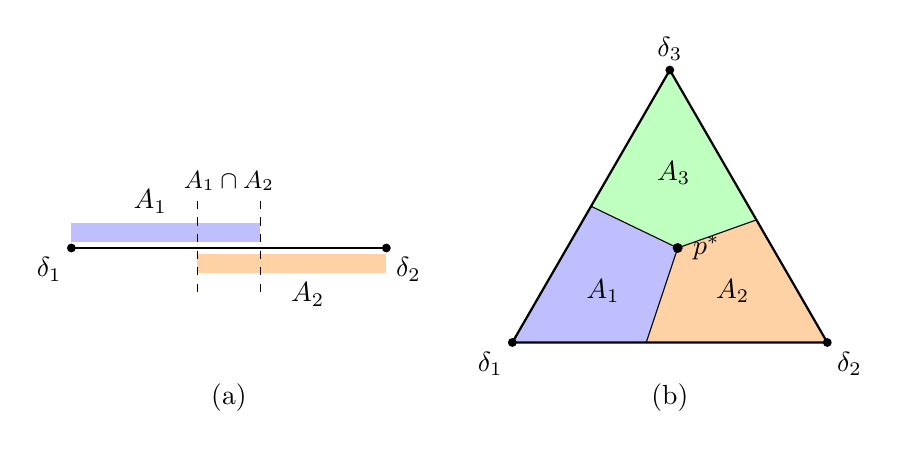
\begin{tikzpicture}
\begin{scope}[yshift=1.2cm]
 \fill[blue!25] (0,0.08) rectangle (2.4,0.32);
 \fill[orange!35] (1.6,-0.32) rectangle (4,-0.08);
 \draw[thick] (0,0) -- (4,0);
 \fill (0,0) circle (1.6pt); \fill (4,0) circle (1.6pt);
 \node[below left] at (0,0) {$\delta_1$};
 \node[below right] at (4,0) {$\delta_2$};
 \node[above] at (1.0,0.32) {$A_1$};
 \node[below] at (3.0,-0.32) {$A_2$};
 \draw[dashed] (1.6,0.6) -- (1.6,-0.6);
 \draw[dashed] (2.4,0.6) -- (2.4,-0.6);
 \node[above] at (2,0.6) {\small $A_1\cap A_2$};
 \node at (2,-1.9) {(a)};
\end{scope}
\begin{scope}[xshift=5.6cm]
 \coordinate (d1) at (0,0); \coordinate (d2) at (4,0); \coordinate (d3) at (2,3.46);
 \coordinate (e12) at (1.7,0); \coordinate (e23) at (3.1,1.557); \coordinate (e13) at (1,1.73);
 \coordinate (c) at (2.1,1.2);
 \fill[blue!25] (d1)--(e12)--(c)--(e13)--cycle;
 \fill[orange!35] (d2)--(e23)--(c)--(e12)--cycle;
 \fill[green!25] (d3)--(e13)--(c)--(e23)--cycle;
 \draw[thick] (d1)--(d2)--(d3)--cycle;
 \draw (e12)--(c) (e23)--(c) (e13)--(c);
 \foreach \p in {d1,d2,d3} \fill (\p) circle (1.6pt);
 \node[below left] at (d1) {$\delta_1$};
 \node[below right] at (d2) {$\delta_2$};
 \node[above] at (d3) {$\delta_3$};
 \node at (1.15,0.65) {$A_1$};
 \node at (2.8,0.65) {$A_2$};
 \node at (2.05,2.15) {$A_3$};
 \fill (c) circle (1.8pt) node[right=2pt] {$p^*$};
 \node at (2,-0.7) {(b)};
\end{scope}
\end{tikzpicture}
\caption{Lemma~\ref{lem:kkm} for $|F|=2$ and $|F|=3$. Each vertex $\delta_\omega$ lies in $A_\omega$, and each face of the simplex is covered by the sets indexed by its vertices. (a)~Closed sets $A_1\ni\delta_1$ and $A_2\ni\delta_2$ that cover the segment must meet. (b)~Each edge is covered by the two sets of its endpoints; the three closed sets have a common point $p^*$.}
\label{fig:kkm}
\end{figure}

\begin{figure}[ht]
\centering
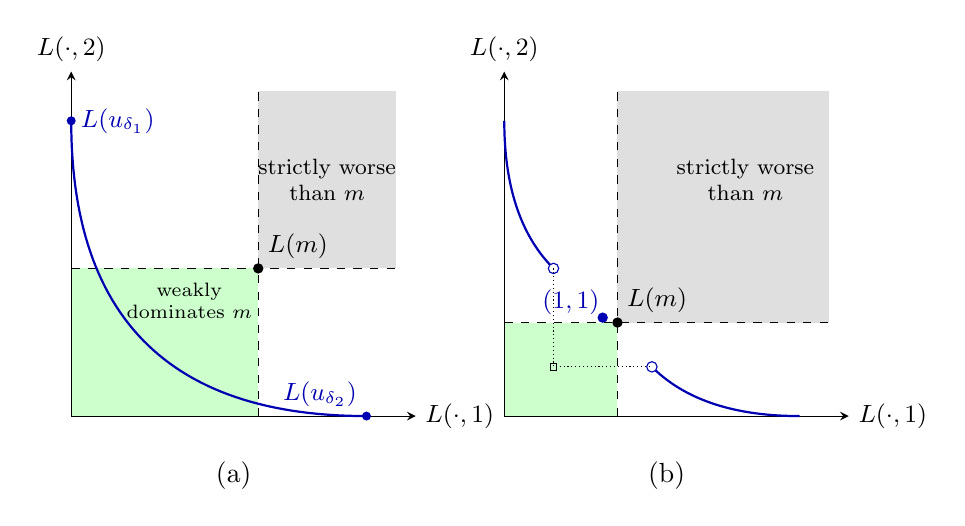
\begin{tikzpicture}[scale=1.25,>=stealth]
\begin{scope}
 \fill[gray!25] (1.9,1.5) rectangle (3.3,3.3);
 \fill[green!20] (0,0) rectangle (1.9,1.5);
 \draw[->] (0,0) -- (3.5,0) node[right] {\small $L(\cdot,1)$};
 \draw[->] (0,0) -- (0,3.5) node[above] {\small $L(\cdot,2)$};
 \draw[dashed] (1.9,0) -- (1.9,3.3);
 \draw[dashed] (0,1.5) -- (3.3,1.5);
 \draw[thick,blue!70!black,domain=0:1,samples=60] plot ({3*(1-\x)^2},{3*\x^2});
 \fill[blue!70!black] (0,3) circle (1.3pt) node[right] {\small $L(u_{\delta_1})$};
 \fill[blue!70!black] (3,0) circle (1.3pt) node[above left] {\small $L(u_{\delta_2})$};
 \fill (1.9,1.5) circle (1.5pt) node[above right] {\small $L(m)$};
 \node[align=center,font=\footnotesize] at (2.6,2.4) {strictly worse\\than $m$};
 \node[align=center,font=\scriptsize] at (1.2,1.17) {weakly\\dominates $m$};
 \node at (1.65,-0.6) {(a)};
\end{scope}
\begin{scope}[xshift=4.4cm]
 \fill[gray!25] (1.15,0.95) rectangle (3.3,3.3);
 \fill[green!20] (0,0) rectangle (1.15,0.95);
 \draw[->] (0,0) -- (3.5,0) node[right] {\small $L(\cdot,1)$};
 \draw[->] (0,0) -- (0,3.5) node[above] {\small $L(\cdot,2)$};
 \draw[dashed] (1.15,0) -- (1.15,3.3);
 \draw[dashed] (0,0.95) -- (3.3,0.95);
 \draw[thick,blue!70!black,domain=0.5:1,samples=40] plot ({2*(1-\x)^2},{1+2*\x^2});
 \draw[thick,blue!70!black,domain=0:0.5,samples=40] plot ({1+2*(1-\x)^2},{2*\x^2});
 \draw[blue!70!black,fill=white] (0.5,1.5) circle (1.5pt);
 \draw[blue!70!black,fill=white] (1.5,0.5) circle (1.5pt);
 \fill[blue!70!black] (1,1) circle (1.5pt) node[above left,inner sep=1pt] {\small $(1,1)$};
 \fill (1.15,0.95) circle (1.5pt) node[above right] {\small $L(m)$};
 \draw[densely dotted] (0.5,1.5) -- (0.5,0.5) -- (1.5,0.5);
 \draw (0.5,0.5) node[draw,rectangle,inner sep=1.2pt] {};
 \node[align=center,font=\footnotesize] at (2.45,2.4) {strictly worse\\than $m$};
 \node at (1.65,-0.6) {(b)};
\end{scope}
\end{tikzpicture}
\caption{(a)~Corollary~\ref{cor:S} for two worlds, for a ranking generated by a loss. The chosen profiles $p\mapsto L(u_p)$ run from $L(u_{\delta_1})$, left of the vertical dashed line, to $L(u_{\delta_2})$, below the horizontal one. The sets $A_1$ and $A_2$ in the proof consist of the $p$ whose profiles lie left of, respectively below, these lines. Since every $u_p$ is competitive on $\supp p$, the curve avoids the grey quadrant, so it must meet the lower-left quadrant, where profiles weakly dominate $m$. (b)~Example~4 of Schervish, Seidenfeld and Kadane~\cite{SSK09}, with $u_p=p$ and $m=(0.6,0.7)$, so $L(m)=(1.15,0.95)$. As $p$ passes through $(\tfrac12,\tfrac12)$, the chosen profiles jump from near $(0.5,1.5)$ to $(1,1)$ to near $(1.5,0.5)$. The curve avoids the grey quadrant but skips the lower-left one. Lower semicontinuity would force the profile at $(\tfrac12,\tfrac12)$ to lie at or below $(0.5,0.5)$, the boxed corner, which is inside that quadrant. Condition (S) fails too: the set of $p$ whose chosen model does at least as well as $m$ at world~$2$ contains every $p$ with $p_1<\tfrac12$ but not $(\tfrac12,\tfrac12)$, so it is not closed.}
\label{fig:profiles}
\end{figure}

\subsection{\texorpdfstring{$\Omega$}{Omega} infinite}\label{sec:infinite}
For arbitrary $\Omega$ we use (LA), (I) and (B$_\infty$), and reduce to the finite case by compactness.

\begin{theorem}\label{thm:infinite-bounds}
Let $\Omega$ be arbitrary and assume that $L$ satisfies (LA), (I) and (B$_\infty$). Then every $m\in\M_L$ is weakly dominated by some $c_\theta$ with $\theta\in\Theta$, and conclusions (b) and (c) of Theorem~\ref{thm:main} hold.
\end{theorem}
\begin{proof}
Choose $m\in\M_L$. For $\omega\in\Omega$ let $\Theta_\omega=\{\theta\in\Theta:c_\theta\preceq_\omega m\}$, which is closed by (I). For $F\in\F$ let
\[
 T_F=\{\theta:c_\theta\preceq_\omega m\text{ for all }\omega\in F\} = \bigcap_{\omega\in F}\Theta_\omega,
\]
a finite intersection of closed sets, hence closed. For $\omega\in F$ put $A^F_\omega=\{p\in\Delta_F:m\in B_{F,\omega}(p)\}$. These sets are closed by (B$_\infty$), and by clause (ii) every $p\in\Delta_F$ lies in $A^F_\omega$ for some $\omega\in\supp p$. Lemma~\ref{lem:kkm} gives $p_F$ with $m\in B_{F,\omega}(p_F)$ for every $\omega\in F$, and clause (i) gives $\theta$ with $c_\theta\preceq_\omega m$ for every $\omega\in F$. So $T_F\ne\varnothing$.

For any $F_1,\dots,F_k\in\F$, some $G\in\F$ contains their union, and then $\varnothing\ne T_G\subseteq T_{F_1}\cap\dots\cap T_{F_k}$. So the closed sets $T_F$, $F\in\F$, have the finite intersection property. Since $\Theta$ is compact, $\bigcap_{F\in\F}T_F\neq \varnothing$. (Otherwise the open sets $\Theta\setminus T_F$ would cover $\Theta$, and some finite subfamily $\Theta\setminus T_{F_1},\dots,\Theta\setminus T_{F_k}$ would cover it, so that $T_{F_1}\cap\dots\cap T_{F_k}=\varnothing$.) Choose $\theta_m\in\bigcap_{F\in\F}T_F$ and $\omega\in\Omega$. Some $F\in\F$ contains $\omega$, and $\theta_m\in T_F$, so $c_{\theta_m}\preceq_\omega m$. Since $\omega$ was arbitrary, $c_{\theta_m}\preceq m$. Conclusions (b) and (c) follow from this exactly as in the proof of Theorem~\ref{thm:main}.
\end{proof}

\begin{corollary}\label{cor:infinite}
Let $\Omega$ be arbitrary and assume that $L$ satisfies (LA), (I) and (S$_\infty$). Then the conclusions of Theorem~\ref{thm:infinite-bounds} hold.
\end{corollary}
\begin{proof}
Proposition~\ref{prop:SBinfty} and Theorem~\ref{thm:infinite-bounds}.
\end{proof}
Again the proofs use no property of the relations $\preceq_\omega$. The topology enters twice: through the closed sets of (B$_\infty$), for the KKM step on each finite set of worlds, and through the compactness of $\Theta$ in (I), which combines the finitely many worlds of each $F$ into one weak dominator for all worlds.

\subsection{Results that use transitivity}\label{sec:preorder}
Two further conclusions need transitivity of the relations $\preceq_\omega$.

\begin{proposition}\label{prop:profiles}
Let $L$ be a preorder ranking satisfying the conclusion of Theorem~\ref{thm:main}(a): every model is weakly dominated by some member of $\C_L$. Then
\[
 \U_L=\{m\in\M_L:m\approx c\text{ for some }c\in\C_L\},
\]
and every $m\in\M_L\setminus\U_L$ is dominated by some member of $\C_L$. Writing $K$ and $U_R$ for the sets of profiles of members of $\C_L$ and of $\U_L$, this says $U_R=K$.
\end{proposition}
\begin{proof}
By Theorem~\ref{thm:main}(b), every undominated model is tied at every world with some $c\in\C_L$; that proof uses only the stated conclusion. Conversely, let $m\approx c$ with $c\in\C_L$, and suppose $m'\precneqq m$. Then $m'\preceq m\preceq c$, so $m'\preceq c$ by transitivity. If $c\preceq m'$, then $m\preceq c\preceq m'$ would give $m\preceq m'$, contrary to $m'\precneqq m$. So $m'\precneqq c$, contrary to $c\in\C_L$. Hence $m$ is undominated. Finally let $m\notin\U_L$, and let $c\in\C_L$ weakly dominate $m$. Then $m\not\approx c$ by the displayed equality, so $c\precneqq m$.
\end{proof}
Without transitivity the inclusion of $\U_L$ in the displayed set remains (Theorem~\ref{thm:main}(b)), but the reverse inclusion can fail: a model tied at every world with an undominated coherent model can itself be dominated. Under (C) the question does not arise, since then $\U_L=\C_L$.

\begin{example}\label{ex:intransitive}
Let $\Omega$ have a single world, $\M_L=\{c,m,m'\}$ and $\C=\{c\}$. Let $\preceq_\omega$ consist of the pairs $c\preceq_\omega c$, $m\preceq_\omega m$, $m'\preceq_\omega m'$, $c\preceq_\omega m$, $m\preceq_\omega c$, $c\preceq_\omega m'$ and $m'\preceq_\omega m$. This relation is reflexive but not transitive, since $m\preceq_\omega c$ and $c\preceq_\omega m'$ but not $m\preceq_\omega m'$. No model dominates $c$, so $\C_L=\{c\}$. The certificate $B_\omega(p)=\M_L$ at the unique $p\in\Delta$, with realiser $c$, satisfies (B), and (S) holds with $u_p=c$. Now $m\approx c$, but $m'$ dominates $m$, and $c$ dominates $m'$. So $\U_L=\{c\}$, while the set displayed in Proposition~\ref{prop:profiles} is $\{c,m\}$. Condition (C) fails, since $m\approx c$ and $m\notin\C_L$.
\end{example}

\begin{corollary}\label{cor:strict-ordinal}
Let $L$ be a ranking whose relations $\preceq_\omega$ are transitive, satisfying (LA) and either (B) with $\Omega$ finite, or (I) and (B$_\infty$). Let $S\subseteq\Omega$ be nonempty. If some model strictly dominates $m\in\M_L$ on $S$, then some member of $\C_L$ strictly dominates $m$ on $S$.
\end{corollary}
\begin{proof}
Let $m'$ strictly dominate $m$ on $S$. By Theorem~\ref{thm:main} or Theorem~\ref{thm:infinite-bounds}, some $c\in\C_L$ weakly dominates $m'$. Let $\omega\in S$. Then $c\preceq_\omega m'\prec_\omega m$. By transitivity $c\preceq_\omega m$, and $m\preceq_\omega c$ would give $m\preceq_\omega m'$. Hence $c\prec_\omega m$.
\end{proof}
For rankings generated by a loss, Appendix~\ref{sec:real} gives conditions under which a model is strictly, and indeed uniformly, dominated if and only if it is a Bayes model for no prior. Those conditions and that characterisation depend on the numerical values of the losses.

\subsection{A route through admissibility}\label{sec:admissibility}
The theorems above establish (W) through certificates. For rankings whose comparisons at each world are lexicographic in finitely many numbers, there is a second route. It establishes (W) by showing that every model is weakly dominated by an undominated one, and that undominated models are coherent.

Say that $L$ is \emph{lexicographic with $k$ levels} if there are functions $z_{\omega,j}:\M_L\to\R$, for $\omega\in\Omega$ and $j=1,\dots,k$, such that $m\preceq_\omega m'$ if and only if $z_\omega(m)\le_{\mathrm{lex}}z_\omega(m')$, where $z_\omega(m)=(z_{\omega,1}(m),\dots,z_{\omega,k}(m))$ and $\le_{\mathrm{lex}}$ is the lexicographic order on $\R^k$. Write $z(m)=(z_\omega(m))_{\omega\in\Omega}$ and $Z=z(\M_L)\subseteq\R^{\Omega\times\{1,\dots,k\}}$, with the product topology. The relations $\preceq_\omega$ are then complete preorders, and all comparisons depend on $m$ only through $z(m)$.

\begin{lemma}\label{lem:zorn}
Let $L$ be lexicographic with $k$ levels, with $\Omega$ arbitrary, and suppose that $Z$ is compact. Then every model is weakly dominated by an undominated model.
\end{lemma}
\begin{proof}
Fix $m$ and let $D=\{y\in Z:y\preceq z(m)\}$, where $y\preceq y'$ means $y_\omega\le_{\mathrm{lex}}y'_\omega$ for every $\omega$. Let $\mathcal K\subseteq D$ be a chain, viewed as a net decreasing in $\preceq$, and let $y^\infty\in Z$ be a cluster point. Fix $\omega$ and $y^\gamma\in\mathcal K$; we show $y^\infty_\omega\le_{\mathrm{lex}}y^\gamma_\omega$. Along the elements of $\mathcal K$ below $y^\gamma$, the first coordinate at $\omega$ is non-increasing, so $y^\infty_{\omega,1}$ is its infimum. If $y^\infty_{\omega,1}<y^\gamma_{\omega,1}$ we are done. Otherwise every element below $y^\gamma$ has the same first coordinate at $\omega$, so along them the second coordinate is non-increasing, and the same argument applies to it; after at most $k$ steps, $y^\infty_\omega\le_{\mathrm{lex}}y^\gamma_\omega$. So $y^\infty\in D$ is a lower bound of $\mathcal K$. By Zorn's lemma, $D$ has an element $y^*$ such that no $y\in D$ has $y\preceq y^*$ without $y^*\preceq y$. If some $y\in Z$ dominated $y^*$, then $y\preceq y^*\preceq z(m)$ would put $y$ in $D$. So any model $m^*$ with $z(m^*)=y^*$ is undominated, and it weakly dominates $m$.
\end{proof}
So for such rankings, (W) holds as soon as every undominated model belongs to $\C$; then $\U_L=\C_L$. When $Z$ is also convex, undominated models can be identified by a separation argument. We state it for two levels.

\begin{proposition}\label{prop:lexbayes}
Let $\Omega$ be finite and $L$ lexicographic with two levels, written $a_\omega=z_{\omega,1}$ and $b_\omega=z_{\omega,2}$. Suppose that $Z$ is convex, that $a_\omega\ge0$ on $\M_L$ for every $\omega$, and that some model has $a_\omega=0$ at every world. Let $m^*$ be undominated and $W_0=\{\omega:a_\omega(m^*)=0\}$. Then $W_0\ne\varnothing$, and there are $\alpha_\omega\ge0$ for $\omega\notin W_0$ and $\beta_\omega\ge0$ for $\omega\in W_0$, with $\beta\neq0$, such that $m^*$ minimises
\[
 J=\sum_{\omega\in W_0}\beta_\omega b_\omega+\sum_{\omega\notin W_0}\alpha_\omega a_\omega
\]
over the models $m$ with $a_\omega(m)=0$ for every $\omega\in W_0$.
\end{proposition}
\begin{proof}
Let $Z'=\{y\in Z:a_\omega(y)=0\text{ for }\omega\in W_0\}$, which is convex, and use on it the coordinates $y'=((b_\omega)_{\omega\in W_0},(a_\omega,b_\omega)_{\omega\notin W_0})$. Let $P^\circ$ be the open convex cone of vectors $d$ with $d_{b_\omega}<0$ for $\omega\in W_0$ and $d_{a_\omega}<0$ for $\omega\notin W_0$. A point $y\in Z'$ with $y'-z(m^*)'\in P^\circ$ would be strictly better than $z(m^*)$ at every world, so $Z'-z(m^*)$ and $P^\circ$ are disjoint. A separating functional $\lambda\ne0$ satisfies $\lambda\cdot d\le0$ on the closure of $P^\circ$, which forces $\lambda_{b_\omega}\ge0$ for $\omega\in W_0$, $\lambda_{a_\omega}\ge0$ and $\lambda_{b_\omega}=0$ for $\omega\notin W_0$; and $\lambda\cdot(y'-z(m^*)')\ge0$ on $Z'$. This gives the weights. If $\beta=0$, then $J=\sum_{\omega\notin W_0}\alpha_\omega a_\omega\ge0$ on $Z'$, with value $0$ at a model with $a\equiv0$; so $J(m^*)=0$, and $a_\omega(m^*)=0$ for some $\omega\notin W_0$ with $\alpha_\omega>0$, which is impossible. If $W_0$ were empty, $\beta$ would have no coordinates.
\end{proof}
Suppose that each model assigns to each point $s$ of a non-atomic probability space $(H,\mu)$ one of finitely many actions $m(s)$, that the domain consists of all measurable such assignments (so that it is closed under splicing models along measurable subsets of $H$), and that each level has the form $z_{\omega,j}(m)=\int f_{\omega,j}(s,m(s))\,d\mu(s)$ with integrable $f_{\omega,j}$. Then $Z$ is convex and compact, by Lyapunov's convexity theorem applied to the finitely many sets $m^{-1}(a)$. Proposition~\ref{prop:lexbayes} then reduces the dominance conclusion to a check on the minimisers of the functionals $J$: if each is unique up to null sets and coherent, every undominated model is coherent, and Lemma~\ref{lem:zorn} gives (W). This route needs numerical lexicographic structure and convexity of $Z$, which the certificate route does not. It needs no closed sections and no certificates.

\section{Certificates and selections}\label{sec:compare}
This section explains what (B) adds to (S), shows that it is strictly weaker, and records what it does not provide.

\subsection{Two separations}\label{sec:separations}
Condition (S) ties three things together at each index $p$: the index itself, a coherent model chosen for $p$, and the comparisons that model makes. Two of these ties are not needed.

The first concerns the index and the prior that certifies competitiveness. A natural way to verify (S) is to choose for each $p$ a coherent model that is a Bayes model for $p$ (Appendix~\ref{sec:bayes}). But the index need not be the certifying prior. It suffices that the chosen model be a Bayes model for some prior whose support lies within $\supp p$. Section~\ref{sec:conditional} uses this freedom essentially. There ordinary conditioning has no continuous extension to the boundary of the simplex, and no selection with lower semicontinuous losses makes every chosen model a Bayes model for its own index (Example~\ref{ex:conditional}). The construction instead assigns each index $p$ a certifying prior $q_0$ that gives zero weight to cells of small probability, while the conditional reports given those cells move continuously towards fixed fallback probabilities. That construction still satisfies (S).

The second separation, which (B) makes, concerns the chosen model and the comparisons that must vary regularly. Under (S), the closed sets used in the KKM argument are the full comparison sections $\{p:u_p\preceq_\omega m\}$ of the chosen models. Under (B), they are the sections of the certificates. A realiser of the certificates may make further comparisons that do not vary in a closed way, and the realiser itself may jump as $p$ varies. The dominance argument never looks at those further comparisons. So regularly varying certificates may be realised by coherent models that change discontinuously, even when no choice of coherent models has closed full comparison sections.

Neither separation weakens the other requirements. At each vertex $\delta_\omega$ of the simplex, (B2) puts every evaluable model into the certificate at $\omega$, and (B3) then requires a coherent undominated model that matches or beats every model at $\omega$. At each interior index a single realiser must meet all the certificates at every world.

\subsection{Condition (B) is strictly weaker than (S)}\label{sec:strict-weakening}
The next example has three worlds and is generated by a loss. For a ranking generated by a loss and nonempty $S\subseteq\Omega$, let $K^S$ be the set of loss profiles of coherent models that are competitive on $S$, that is, that no model strictly dominates on $S$.

\begin{proposition}\label{prop:threeworld}
Let $\Omega=\{1,2,3\}$ and $b(t)=\max\{0,\,0.1-5|t-\tfrac12|\}$. Let
\[
 K=\{k(t)=(t+b(t),\ 1-t+b(t),\ 1-5b(t)):t\in[0,1]\},
\]
let $\C$ consist of one model with each profile in $K$, and let $\M_L$ consist of $\C$ together with one further model $z$ with profile $(2,2,2)$. Then (LA) and (C) hold, $\C_L=\C$, $K$ is compact and connected, each world has a coherent model that matches or beats every model there, and $z$ is dominated by every coherent model. Condition (B) holds, but (S) cannot be met.
\end{proposition}
\begin{proof}
\emph{(LA) and (C).} Suppose $k(t)\le k(t')$. The third coordinate gives $b(t)\ge b(t')$, and the sum of the first two gives $b(t)\le b(t')$. So $b(t)=b(t')$, and then the first two coordinates give $t=t'$. Every coordinate of every $k(t)$ is at most $1$, so every coherent model strictly dominates $z$, and $z$ dominates no model. Hence no model dominates a coherent model, $\C_L=\C$, and $z$ is tied at every world with no coherent model, which gives (C).

\emph{The sets $K^S$.} Since $z$ strictly dominates nothing, only coherent profiles matter. The first coordinate $t+b(t)$ is least, with value $0$, only at $t=0$, so $K^{\{1\}}=\{k(0)\}$; similarly $K^{\{2\}}=\{k(1)\}$. The third coordinate is least only at $t=\tfrac12$, so $K^{\{3\}}=\{k(\tfrac12)\}$. Next, $k(t')$ strictly dominates $k(t)$ on $\{1,2\}$ iff $|t'-t|<b(t)-b(t')$. No $k(t)$ with $b(t)=0$ is strictly dominated on $\{1,2\}$. For $t\in(0.48,0.5]$, $t'=0.48$ gives $t-0.48<5(t-0.48)=b(t)$; symmetrically for $t\in[0.5,0.52)$. So $K^{\{1,2\}}$ is the union of the disjoint closed sets $\{k(t):t\le0.48\}\ni k(0)$ and $\{k(t):t\ge0.52\}\ni k(1)$.

\emph{(S) cannot be met.} Suppose (S) held, with selection map $u$. On the edge from $\delta_1$ to $\delta_2$ we have $L(u_p)\in K^{\supp p}\subseteq K^{\{1,2\}}$, with $L(u_{\delta_1})=k(0)$ and $L(u_{\delta_2})=k(1)$. A point $k(t)$ of $K^{\{1,2\}}$ has first coordinate at most $0.48$ iff $t\le0.48$, and second coordinate at most $0.48$ iff $t\ge0.52$. Let $m_1$ and $m_2$ be the coherent models with profiles $k(0.48)$ and $k(0.52)$. Then the sets $\{p:u_p\preceq_1 m_1\}$ and $\{p:u_p\preceq_2m_2\}$, intersected with the edge, are closed by (S), disjoint, cover the edge, and contain $\delta_1$ and $\delta_2$ respectively. This contradicts connectedness of the edge.

\emph{(B) holds.} $K$ is the continuous image of $[0,1]$, so it is compact and connected, and every model is weakly dominated by a coherent one. Proposition~\ref{prop:necessary} in Appendix~\ref{sec:finite} therefore gives certificates satisfying (B) on the whole simplex.
\end{proof}
So (S) is not necessary for the conclusions of Theorem~\ref{thm:main}, even when the coherent profiles form a compact connected set and every world has a coherent model that matches or beats every model there.

The certificates given by Proposition~\ref{prop:necessary} are defined from the conclusion of the theorem, so they do not explain why that conclusion holds (Section~\ref{sec:limits}). On the edge where (S) fails, the mechanism can be seen directly.

\begin{remark}\label{rem:threeworld-bounds}
In Proposition~\ref{prop:threeworld}, describe certificates numerically: for a point $Q\in\R^\Omega$, let the certificate at $\omega$ consist of the models $m$ with $Q(\omega)\le L(m,\omega)$. The obstruction to (S) was the gap in $K^{\{1,2\}}$ between $k(0.48)=(0.48,0.52,1)$ and $k(0.52)=(0.52,0.48,1)$. Certificates can cross it through the corner $(0.52,0.52,1)$. Along the edge from $\delta_1$ to $\delta_2$, let $Q(p)$ follow $k(t)$ for $t\le0.48$, then the segment from $k(0.48)$ to $(0.52,0.52,1)$, then the segment from there to $k(0.52)$, and then $k(t)$ for $t\ge0.52$. This is a continuous path from $k(0)$ to $k(1)$; parametrise it continuously by the position of $p$ on the edge. Then each set $\{p:Q(p)(\omega)\le L(m,\omega)\}$ is closed, which is (B1) on the edge. We check these certificates only on that edge. Each point of the two segments lies weakly above $k(0.48)$ or $k(0.52)$, which gives (B3), with realiser of profile $k(0.48)$ on the first segment and $k(0.52)$ on the second; on the rest of the path the realiser is the coherent model with profile $Q(p)$. No profile strictly dominates such a point on $\{1,2\}$: that would need $t+b(t)<0.52$ and $1-t+b(t)<0.52$, that is, $|t-\tfrac12|<0.02-b(t)$, which is impossible both where $b(t)=0$ and where $b(t)=0.1-5|t-\tfrac12|>0$. The other points of the path lie in $K^{\{1,2\}}$, and the endpoints $k(0)\in K^{\{1\}}$ and $k(1)\in K^{\{2\}}$. Since rankings generated by losses have no incomparabilities, this gives (B2) at every point of the edge. The certificates vary continuously, but the realiser jumps at the corner, from the group $t\le0.48$ to the group $t\ge0.52$. Some jump is unavoidable for any certificates satisfying (B) on this edge. By (B2) and (B3) every realiser at $p$ is competitive on $\supp p$, so on the edge its profile lies in $K^{\{1,2\}}$, at $\delta_1$ it is $k(0)$, and at $\delta_2$ it is $k(1)$. If some choice of realisers had closed full comparison sections, it would be a selection map satisfying (S) on the edge, which the proof of Proposition~\ref{prop:threeworld} excludes. Only the comparisons of the realisers with models other than those their certificates list fail to vary in a closed way, and the argument does not need them.

No certificates of the form supplied by Bayes models (Lemma~\ref{lem:bayesbounds}) satisfy (B) on this edge. The coherent Bayes models for probabilities on $\{1,2\}$ are $k(0)$, $k(1)$, and, for $(\tfrac12,\tfrac12)$, the $k(t)$ with $b(t)=0$. So certificates of that form have $(Q(p)(1),Q(p)(2))$ in $\{Q(p)(1)\le0.48,\ Q(p)(2)\ge0.52\}$ or in $\{Q(p)(2)\le0.48,\ Q(p)(1)\ge0.52\}$. By (B1), applied with the models of profiles $k(0.48)$ and $k(0.52)$, the sets of $p$ with $Q(p)(1)\le0.48$ and with $Q(p)(2)\le0.48$ are closed. They are disjoint, cover the edge, and contain $\delta_1$ and $\delta_2$ respectively, which is impossible because the edge is connected.
\end{remark}

The example concerns a continuum of loss profiles on finitely many worlds and uses no structure of the models. It shows that the general technical condition can be weakened from (S) to (B) without losing the dominance conclusion. It is not a construction for any particular class of coherent models.

\subsection{What certificates do not provide}\label{sec:limits}
Condition (B) is a sufficient condition, and its value as an explanation depends on how the certificates are obtained.

First, (B) is not the weakest condition from which the conclusions follow. The conclusion of Theorem~\ref{thm:main}(a) is itself necessary and sufficient for it, and for compact sets of coherent loss profiles on finitely many worlds, (B) is equivalent to it (Proposition~\ref{prop:necessary}). The certificates used to prove that equivalence are built from the conclusion. Remark~\ref{rem:elementary} shows that with them the implication from (B2) to coherent weak dominance needs no fixed-point argument at all. Such certificates merely repackage a dominance conclusion that is already known.

Secondly, certificates should not be allowed to depend on the rival. The KKM argument fixes one rival $m$ at a time. If each rival $m$ could have its own certificates, closed in $p$, it would suffice for $m$ alone to be covered and met. But if some coherent $c$ already weakly dominates $m$, the constant certificate $B_\omega(p)=\{m\}$ with realiser $c$ does this. So that weakening is equivalent to the conclusion it is meant to explain.

The substantive use of Theorem~\ref{thm:main} is therefore to supply certificates by some independent route, and to prove the dominance conclusion from them. The applications in Section~\ref{sec:apps} do this through selections that satisfy (S) or (S$_\infty$), checked through Bayes models. Certificates given by Bayes models of priors supported in $\supp p$ are a second route (Lemma~\ref{lem:bayesbounds}). Remark~\ref{rem:threeworld-bounds} shows that they do not always suffice.

\section{Coherence and rational permissibility}\label{sec:argument}

What do these results tell us (if anything) about whether coherent models are rationally preferable to incoherent models?

Models are used for some purpose or other. For example, a set of precise forecasts for a range of weather events might be used to estimate whether those events will occur or not. A set of interval forecasts for a range of public health events might be used to guide policymakers in their decisions. Whatever the purpose or task, we assume that models perform better or worse in different states of the world. And rankings measure some property or other relevant to evaluating how well they perform in those states.

Note, however, that it may not be perfectly determinate what \textit{performing well} amounts to, even once we specify the purpose or task of interest carefully. This may be true for a variety of reasons. Here is an especially clear one though: good performance is often multi-dimensional. Running a restaurant well, for example, involves putting out creative dishes, executing those dishes consistently, serving customers promptly, minimising costs, etc. There may be a number of different reasonable ways to weigh up overall performance as a function of performance in these various dimensions. Each one yields a different notion of \textit{performing well}.

In Section~\ref{sec:axioms}, we assumed that the set $\mathfrak L$ of rankings is a putatively complete class, in the sense that it contains all and only the rankings that measure how well the models in $\M$ perform a given task, and do so in a reasonable fashion. We allowed that each ranking $L\in\mathfrak L$ might only evaluate a certain subset of models, $\M_L\subseteq\M$. But we assumed that as a class, $\mathfrak L$ collectively evaluates every model (\textit{i.e.}, $\M=\bigcup_{L\in\mathfrak L}\M_L$). This was assumption (E).

The verdicts of the \textit{entire class of reasonable rankings} are what matters for whether or not it is rationally permissible to use a given model for some purpose or not. In particular, we assume:
\begin{enumerate}[label=\textbf{(D)},leftmargin=*]
\item \textbf{Dominance.} A model $m\in\M$ is irrational if, for every $L\in\mathfrak L$ with $m\in\M_L$, there is some $m_L^\prime\in\U_L$ with $m_L^\prime\precneqq_L m$. A model $m$ is rationally permissible if $m\in\U_L$ for some $L\in\mathfrak L$.
\end{enumerate}

This says that it is irrational to use a model $m$ for a given purpose or task if on \textit{any} reasonable way of measuring good performance at that task (any $L\in\mathfrak L$), there is some alternative $m_L^\prime$ that dominates it, in the sense that it could not possibly do worse and might do better (according to $L$); moreover the alternative does not itself suffer this defect (it is undominated, \textit{i.e.}, $m_L^\prime\in\U_L$). On the flip side, it is rationally permissible to use a model for a purpose if there is \textit{some} reasonable way of measuring good performance that renders $m$ free of the defect of domination. Of course, some particular evaluator (a single forecaster or decision-maker, a governmental organisation, etc.) might care about some ways of measuring good performance and not others. In that case, we must tailor $\mathfrak L$ appropriately.

With this dominance principle in hand, we can provide a general recipe for how to argue that the rationally permissible models are exactly the coherent ones.
\begin{enumerate}[label=\textbf{(P\arabic*)},leftmargin=*]
\item $\mathfrak L$ satisfies (E) and (A), and every $L\in\mathfrak L$ satisfies (LA), (C), and either (B) (if $\Omega$ is finite) or (I) and (B$_\infty$).
\item \textbf{Dominance} (D).
\item Proposition~\ref{prop:permissible}.
\item[\textbf{(P4)}] The rationally permissible models are exactly the coherent ones, and every incoherent model is irrational.
\end{enumerate}

\begin{proposition}\label{prop:permissible}
Suppose that every $L\in\mathfrak L$ satisfies (LA) and either (B), with $\Omega$ finite, or (I) and (B$_\infty$). Then, for every $L\in\mathfrak L$:
\begin{enumerate}[label=(\alph*)]
\item every $m\in\U_L$ is tied at every world with some $c\in\C_L$;
\item if $L$ satisfies (C), then $\U_L=\C_L$, and every $m\in\M_L\setminus\C_L$ is dominated by some $c\in\C_L$;
\item if $L$ is a preorder ranking, then $\U_L=\{m\in\M_L:m\approx_L c\text{ for some }c\in\C_L\}$, and every $m\in\M_L\setminus\U_L$ is dominated by some $c\in\C_L$.
\end{enumerate}
Suppose further that every $L\in\mathfrak L$ satisfies (C) or is a preorder ranking. Then a model $m\in\M$ lies outside $\bigcup_{L\in\mathfrak L}\U_L$ if and only if, for every $L\in\mathfrak L$ with $m\in\M_L$, some $m'\in\U_L$ has $m'\precneqq_L m$. If (A) holds, then $\C\subseteq\bigcup_{L\in\mathfrak L}\U_L$, with equality if every $L\in\mathfrak L$ satisfies (C).
\end{proposition}
\begin{proof}
Parts (a) and (b) are Theorem~\ref{thm:main} and Theorem~\ref{thm:infinite-bounds}. Part (c) is Proposition~\ref{prop:profiles}. If $m\notin\bigcup_L\U_L$, then $m\notin\U_L$ for every $L$ with $m\in\M_L$; by (b) or (c), some member of $\C_L\subseteq\U_L$ dominates $m$ relative to each such $L$. Conversely, if $m\in\U_L$ for some $L$, then no model dominates $m$ relative to that $L$. By (A), $\C=\bigcup_L\C_L\subseteq\bigcup_L\U_L$. If every $L$ satisfies (C), then (b) gives $\U_L=\C_L$ for every $L$, and so $\bigcup_L\U_L=\bigcup_L\C_L=\C$.
\end{proof}
Without (C) and without transitivity, a model can lie outside $\U_L$ while being tied at every world with an undominated coherent model, and then the coherent dominators supplied by the theorems need not dominate it.

\begin{proposition}\label{prop:permissible-equivalence}
Suppose that every $L\in\mathfrak L$ is a preorder ranking satisfying the hypotheses of Proposition~\ref{prop:permissible}. Let $\sim$ be an equivalence relation on $\M$, and put $[X]:=\{m\in\M:m\sim x\text{ for some }x\in X\}$ for $X\subseteq\M$. If every $L\in\mathfrak L$ satisfies
\begin{equation}\tag{C$_\sim$}\label{eq:identification-equivalence}
 \{m\in\M_L:m\approx_L c\text{ for some }c\in\C_L\}
 =\M_L\cap[\C_L],
\end{equation}
then $\bigcup_{L\in\mathfrak L}\U_L=\bigcup_{L\in\mathfrak L}(\M_L\cap[\C_L])\subseteq[\C]$. If, in addition,
\begin{equation}\tag{A$_\sim$}\label{eq:equivalence-coverage}
 [\C]\subseteq\bigcup_{L\in\mathfrak L}(\M_L\cap[\C_L]),
\end{equation}
then $\bigcup_{L\in\mathfrak L}\U_L=[\C]$. Condition (A$_\sim$) follows from (A) if every $\M_L$ is closed under $\sim$, or if $\C$ is. When $\sim$ is equality, (C$_\sim$) is (C) and (A$_\sim$) is (A).
\end{proposition}
\begin{proof}
By Proposition~\ref{prop:permissible}(c) and (C$_\sim$), $\U_L=\M_L\cap[\C_L]$ for every $L$, and $\M_L\cap[\C_L]\subseteq[\C]$ because $\C_L\subseteq\C$. (A$_\sim$) gives the reverse inclusion. If every $\M_L$ is closed under $\sim$ and $m\sim c\in\C$, choose $L$ with $c\in\C_L$ by (A); then $m\in\M_L\cap[\C_L]$. If $\C$ is closed under $\sim$, then $[\C]=\C=\bigcup_L\C_L\subseteq\bigcup_L(\M_L\cap[\C_L])$ by (A). When $\sim$ is equality, $[X]=X$. Then (C$_\sim$) says that every $m\in\M_L$ tied at every world with a member of $\C_L$ belongs to $\C_L$, which is (C), and (A$_\sim$) says that $\C\subseteq\bigcup_L\C_L$, which, since each $\C_L\subseteq\C$, is (A).
\end{proof}


\section{Some applications of interest}\label{sec:apps}
In the applications below, $\M_L$ is the stated evaluation domain and $\C$ is the stated, independently specified coherent class. Each ranking is generated by a loss function, and we use the notation and results of Appendix~\ref{sec:real}, in particular Lemma~\ref{lem:bayes-choice}. Each application verifies (S) or (S$_\infty$), and hence (B) or (B$_\infty$), through selections that make Bayes choices. We prove that every member of $\C$ is undominated, so that $\C_L=\C$. This verifies (LA) for the loss at hand; it verifies the family-wide condition (A) only when the losses under consideration collectively cover the intended coherent class. Here $K=L(\C_L)=L(\C)$.
\subsection{Proper scores on finite domains}\label{sec:proper}
Let $\Omega$ be finite, $\C=\Delta\subseteq\M_L$, and let each $p\mapsto L(p,\omega)$ be lower semicontinuous on $\Delta$. Assume \emph{strict propriety relative to $\M_L$}: for every $p\in\Delta$, the model $p$ is a Bayes model for $p$ over all of $\M_L$, and every Bayes model for $p$ has profile $L(p)$. Then every $p\in\C$ is undominated, since a model weakly dominating $p$ is a Bayes model for $p$ and must have its profile. Hence $\C_L=\C$ and (LA) holds. The selection map $p\mapsto c_p=p$ satisfies (S), and it makes Bayes choices (Lemma~\ref{lem:bayes-choice}). So, by Corollary~\ref{cor:S} and Proposition~\ref{prop:profiles}, $U_R=K$. If, for every $p$, $p$ is the only Bayes model for $p$, then $\C$ is closed under equal profiles and $\U_L=\C$. Then also no incoherent model is a Bayes model for any prior. Moreover $V(p)=\sum_\omega p_\omega L(p,\omega)$ is finite when $\M_L$ has more than one element, since $V(p)=\infty$ would make every model a Bayes model for $p$. So if every probability has finite losses, or each $p\mapsto L(p,\omega)$ is continuous on $\Delta$, Corollary~\ref{cor:strict} (in the first case) and Proposition~\ref{prop:strict-general} (in the second) show that every incoherent model is uniformly dominated by a coherent one.

This contains Pettigrew's Theorem~1~\cite{Pettigrew}. There $\Omega$ is finite, the models are the credence functions on all subsets of $\Omega$, and the coherent ones are the probabilities, which correspond to the points of $\Delta$. His strict propriety says that $p$ is the only Bayes model for $p$ (reading expected inaccuracies with $0\cdot\infty=0$), and his continuity of each $L(\cdot,\omega)$ on all credence functions implies continuity on the probabilities. His conclusion is that every incoherent credence is strictly dominated by a probability. Continuity cannot simply be dropped~\cite{SSK09}; the discontinuous strictly proper score of~\cite[Example~4]{SSK09} is not lower semicontinuous on the probabilities.

The finite-forecast theorem of Predd et al.~\cite[Theorem~1]{Predd} is also recovered. Summing a continuous strictly proper binary score over finitely many events gives a loss on a finite set of truth-value patterns. Each probability on those patterns has its vector of event probabilities as its unique Bayes report, and the reports have continuous losses. Proposition~\ref{prop:strict-general} therefore gives strict dominance of every incoherent forecast by a coherent forecast. Appendix~\ref{sec:forecasts} gives the reduction, including scores that can take infinite values. It also allows a different, possibly merely proper, continuous score for each event, which recovers \cite[Theorem~2, Conclusion~3]{SSK09} for unconditional forecasts. These finite-score applications recover known results; the next application gives the infinite-domain improvement.

\subsection{Probabilism on arbitrary domains}\label{sec:nielsen} Let $\Omega$ be any nonempty set, $\M_L=[0,1]^{2^\Omega}$ the credence functions on its subsets, and $\C$ the finitely additive probabilities, which form a compact set in the topology of pointwise convergence on subsets. On $\C$ this is the weak-star topology of Section~\ref{sec:conditional}, since bounded functions are uniform limits of simple functions. Let $L:\M_L\times\Omega\to[0,\infty]$, and for $q\in\C$ let $E_q$ be the expectation of $[0,\infty]$-valued functions used by Nielsen~\cite[Appendix A]{Nielsen}: $E_qf$ is the supremum of $q(h)$ over bounded $h\le f$. 
\begin{theorem}\label{thm:nielsen}
Assume \emph{quasi-strict propriety}: $E_qL(q,\cdot)\le E_qL(m,\cdot)$ for every $q\in\C$ and $m\in\M_L$, strictly when $m\notin\C$. Assume also that $q\mapsto L(q,\omega)$ is lower semicontinuous on $\C$ for every world $\omega$. Then the undominated models are exactly the finitely additive probabilities, and every other model is dominated by a probability. If in addition each probability has bounded loss across worlds, every other model is uniformly dominated by a probability.
\end{theorem}
Quasi-strict propriety says that each probability regards its own report as optimal and regards every non-probabilistic report as strictly worse in expectation. Other probabilities may tie. The regularity condition concerns the loss at one fixed world as the probability report varies. It does not require continuity of expected loss for every prior. The additional boundedness condition allows a different bound for each probability; it does not require one bound for all models.
\begin{proof}


First we prove $\C_L=\C$, and hence (LA), adapting Nielsen's proof of his Theorem~2~\cite{Nielsen}. Suppose $L(m)\le L(q)$ with $q\in\C$ and $L(m,w)<L(q,w)$. Then $E_qL(m,\cdot)\le E_qL(q,\cdot)$, which is finite because quasi-strict propriety gives $E_qL(q,\cdot)<E_qL(m',\cdot)$ for any $m'\notin\C$; so equality holds, and $L(m,w)$ is finite. For $n\ge2$ put $q_n=\frac1n\delta_w+(1-\frac1n)q$. Expectations are linear in the probability~\cite[Appendix~A, Proposition~1]{Nielsen}, so quasi-strict propriety at $q_n$ and at $q$ gives $\frac1nL(m,w)+(1-\frac1n)E_qL(m,\cdot)\ge\frac1nL(q_n,w)+(1-\frac1n)E_qL(q,\cdot)$, that is, $L(q_n,w)\le L(m,w)$. Lower semicontinuity gives $L(q,w)\le L(m,w)$, a contradiction. For (I) take $\Theta=\C$ and $c_q=q$. For (S$_\infty$) let $\F$ consist of all finite nonempty sets and let $\sigma_F(p)$ be $p$, viewed as a member of $\C$. Quasi-strict propriety makes $\sigma_F(p)$ a Bayes model for $p$, so Lemma~\ref{lem:bayes-choice} applies. If $L(m)=L(q)$ with $q\in\C$, then $E_qL(m,\cdot)=E_qL(q,\cdot)$, so $m\in\C$. Corollary~\ref{cor:infinite} completes the argument.

\emph{Uniform dominance.} With local boundedness, every $m\notin\C$ is uniformly dominated. For $q\in\C$ put $D(q):=E_qL(m,\cdot)-E_qL(q,\cdot)$, which lies in $(0,\infty]$ by quasi-strict propriety. By local boundedness, $D$ is lower semicontinuous on $\C$~\cite[Lemma~3]{Nielsen}: $q\mapsto E_qL(m,\cdot)$ is a supremum of the continuous maps $q\mapsto q(h)$ over bounded $h\le L(m,\cdot)$, and, by quasi-strict propriety, $E_qL(q,\cdot)=\min_{q'\in\C}E_qL(q',\cdot)$ is an infimum of maps that are continuous~\cite[Lemma~1]{Nielsen} because each $L(q',\cdot)$ is bounded. So $D$ attains a positive minimum on the compact set $\C$; let $\varepsilon$ be a positive real number no larger than it. A finitely supported $p$ is a Bayes model for itself, so $\sum_\omega p_\omega L(m,\omega)=V(p)+D(p)\ge V(p)+\varepsilon$, and Theorem~\ref{thm:margin}, with the choices above and $x=L(m)-\varepsilon$, gives $q\in\C$ with $L(q,\omega)+\varepsilon\le L(m,\omega)$ for every $\omega$. Since $L(q,\cdot)$ is finite, $q$ strictly dominates $m$, and $\inf_\omega(L(m,\omega)-L(q,\omega))\ge\varepsilon$; so $q$ uniformly dominates $m$, and by (LA) it is undominated.
\end{proof}

Nielsen's Theorem~1 concludes strict dominance. In addition to quasi-strict propriety it assumes continuity of $q\mapsto E_pL(q,\cdot)$ for every $p\in\C$, and \emph{local boundedness}, $\sup_\omega L(q,\omega)<\infty$ for every $q\in\C$. His continuity assumption implies continuity at each world by taking $p=\delta_\omega$. Theorem~\ref{thm:nielsen} requires only lower semicontinuity there. Nielsen asks whether local boundedness can be dropped~\cite[\S4.2.1]{Nielsen}. We remove it for ordinary dominance, which permits ties at some worlds. We do not establish strict dominance without it.


Under local boundedness the theorem includes Nielsen's two dominance conclusions. The weakened continuity assumption is also available by adapting his direct proof; the uniform margin is already implicit in that proof~\cite[Appendix~C, (9)]{Nielsen}. Appendix~\ref{sec:direct} gives the finite version of this argument. The distinctive gain from the KKM proof here is ordinary dominance without local boundedness: it avoids minimising the expected-loss gap $D$ on the full space of priors.

\subsection{Conditional reports, including null events}\label{sec:conditional}
Let $E_1,\dots,E_k$ ($k\ge1$) partition $\Omega$ into nonempty cells, and put $F_0=\Omega$ and $F_j=E_j$ for $j\ge1$. The state space $\Omega$ is arbitrary; only the number of cells is finite. For a nonempty set $F$, let $\PP(F)$ be the set of finitely additive probabilities on all subsets of $F$. For $q\in\PP(F)$ and bounded $f$ on $F$, $q(f)$ is the expectation. Give $\PP(F)$ the weak-star topology: $q_\alpha\to q$ iff $q_\alpha(f)\to q(f)$ for every bounded $f$. By Tychonoff's theorem $\PP(F)$ is compact, being a closed subset of $\prod_f[\inf f,\sup f]$. Let
\[
\begin{aligned}
 \Gamma=\bigl\{(q_0,q_1,\dots,q_k):\ & q_0\in\PP(\Omega),\ q_j\in\PP(E_j),\\
 & q_0(\one_{E_j}f)=q_0(E_j)\,q_j(f)\ \text{for all }j\ge1\text{ and bounded }f\text{ on }E_j\bigr\},
\end{aligned}
\]
where $\one_{E_j}f$ is $f$ extended by zero. Thus $q_j$ is the conditional probability when $q_0(E_j)>0$, and a freely chosen probability on $E_j$ when $q_0(E_j)=0$. Each defining identity is a closed condition, so $\Gamma$ is compact.

The difficulty is that ordinary conditioning $p(\cdot\mid E_j)$ has no continuous extension when $p(E_j)$ tends to zero in different ways. We therefore let the certifying prior differ from the index. Cells with very small probability receive zero weight in the certifying prior, while their conditional reports move continuously towards fixed fallback probabilities. Those reports remain coherent even though they no longer affect the certifying expected loss. The following explicit construction implements this idea. It still satisfies (S$_\infty$): what it separates is the index from the certifying prior, not the chosen model from its comparisons (Section~\ref{sec:separations}).

\begin{lemma}\label{lem:section}
Let $F\subseteq\Omega$ be finite and nonempty, $J=\{j:E_j\cap F\ne\varnothing\}$, $\eta=1/(2k)$, $u_j$ uniform on $E_j\cap F$ for $j\in J$, and fix a probability $r_j^0$ on $E_j$ for $j\notin J$. For $p\in\Delta_F$ put
\[
\beta_j=\max(p(E_j)-\eta,0),\qquad \lambda_j=\frac{\beta_j}{\sum_i\beta_i},
\]
\[
r_j=\frac{p|_{E_j}+\max(\eta-p(E_j),0)\,u_j}{p(E_j)+\max(\eta-p(E_j),0)}\ (j\in J),\qquad r_j=r_j^0\ (j\notin J),
\]
and $q_0=\sum_j\lambda_jr_j$. Then $\gamma(p)=(q_0,r_1,\dots,r_k)\in\Gamma$, $p\mapsto\gamma(p)$ is weak-star continuous, and $\supp q_0\subseteq\supp p$.
\end{lemma}
\begin{proof}
Some cell has $p(E_j)\ge1/k$, so $\sum_i\beta_i\ge\eta>0$; the denominators of $r_j$ are at least $\eta$. So $\lambda$ and the $r_j$ ($j\in J$) are continuous in the finitely many $p_\omega$, and the others are constant. Also $q_0(E_j)=\lambda_j$ and $q_0(\one_{E_j}f)=\lambda_jr_j(f)$, so $\gamma(p)\in\Gamma$. If $\lambda_j>0$ then $p(E_j)>\eta$ and $r_j=p|_{E_j}/p(E_j)$. Hence $\supp q_0\subseteq\supp p$.
\end{proof}

\emph{Block losses.} For each $j=0,\dots,k$ fix a set $X_j$ of possible reports for block $j$, a map $\rho_j:\PP(F_j)\to X_j$ (the report stating a given probability), and a block loss $S_j:X_j\times F_j\to[0,\infty)$ with $S_j(x,\cdot)$ bounded for each $x$. Block $0$ is the unconditional block; block $j\ge1$ is the conditional block for $E_j$. A model is a tuple $x=(x_0,\dots,x_k)\in\M_L=X_0\times\dots\times X_k$, and
\[
 L(x,\omega)=S_0(x_0,\omega)+S_j(x_j,\omega)\qquad(\omega\in E_j).
\]
A conditional block counts only at worlds of its own cell. The coherent models are $\rho(\gamma)=(\rho_0(q_0),\dots,\rho_k(q_k))$ for $\gamma\in\Gamma$. For $\gamma\in\Gamma$ and $x\in\M_L$, the identities defining $\Gamma$, applied to $f=S_j(x_j,\cdot)$, give
\begin{equation}\label{eq:blocks}
 q_0\bigl(L(x,\cdot)\bigr)=q_0\bigl(S_0(x_0,\cdot)\bigr)+\sum_{j=1}^kq_0(E_j)\,q_j\bigl(S_j(x_j,\cdot)\bigr).
\end{equation}

\begin{proposition}\label{prop:blocks}
Assume
\begin{enumerate}[label=\textbf{(P)},leftmargin=*]
\item for each $j$ and $q\in\PP(F_j)$, the report $\rho_j(q)$ minimises $x\mapsto q(S_j(x,\cdot))$ over $X_j$, and every minimiser $x$ satisfies $S_j(x,\cdot)=S_j(\rho_j(q),\cdot)$ on $F_j$;
\end{enumerate}
\begin{enumerate}[label=\textbf{(LSC)},leftmargin=*]
\item for each $\omega$, the map $\gamma\mapsto L(\rho(\gamma),\omega)$ is lower semicontinuous on $\Gamma$.
\end{enumerate}
Then $\C_L=\C$, and (LA), (I) and (S$_\infty$) hold with $\Theta=\Gamma$ and $c=\rho$. Hence, by Corollary~\ref{cor:infinite} and Proposition~\ref{prop:profiles}, every model is weakly dominated by a coherent model, and $U_R=K$. If each $\rho_j(q)$ is the \emph{unique} minimiser in (P), then $\U_L=\C$ and every incoherent model is dominated by a coherent one.
\end{proposition}

Condition (P) is a block-by-block optimality and identification requirement. Each probability report minimises its own expected block loss, and any other minimiser must make exactly the same losses at every world of that block. It is stronger than ordinary propriety, which only guarantees a minimum. It leaves room for different reports with identical loss profiles. Condition (LSC) says that coherent systems approaching a limit do not acquire a higher loss at that limit. Neither condition requires a unique Bayes model for the total loss: the total expected loss ignores a conditional block when its event has probability zero.

\begin{proof}
\emph{Admissibility of $\C$.} Let $\gamma\in\Gamma$ and suppose $L(x,\cdot)\le L(\rho(\gamma),\cdot)$. Apply $q_0$ and use \eqref{eq:blocks} for $x$ and for $\rho(\gamma)$. By (P) each term for $x$ is at least the corresponding term for $\rho(\gamma)$, while the totals satisfy the reverse inequality. So all terms are equal. In particular $x_0$ is a minimiser for $q_0$, and (P) gives $S_0(x_0,\cdot)=S_0(\rho_0(q_0),\cdot)$. Cancelling this common block, $S_j(x_j,\omega)\le S_j(\rho_j(q_j),\omega)$ for every $\omega\in E_j$. Apply $q_j$: then $x_j$ is a minimiser for $q_j$, and (P) gives equality on $E_j$. Hence $L(x)=L(\rho(\gamma))$, so no model dominates $\rho(\gamma)$. With unique minimisers the same argument gives $x=\rho(\gamma)$, so $\C$ is closed under equal profiles.

\emph{(I).} $\Gamma$ is compact, and (LSC) gives (I) with lower semicontinuous losses.

\emph{(S$_\infty$).} Let $\F$ be all finite nonempty subsets of $\Omega$ and $\sigma_F$ the map of Lemma~\ref{lem:section}. Write $\sigma_F(p)=(q_0,\dots,q_k)$. By (P), each term on the right of \eqref{eq:blocks} is minimised at $x=\rho(\sigma_F(p))$; terms with $q_0(E_j)=0$ vanish. So $\rho(\sigma_F(p))$ is a Bayes model for $q_0$. Since $q_0$ is finitely supported and $\supp q_0\subseteq\supp p$, Lemma~\ref{lem:bayes-choice} gives (S$_\infty$). Corollary~\ref{cor:infinite} gives the conclusions.
\end{proof}
The proof of admissibility treats a null cell ($q_0(E_j)=0$) like any other: on $E_j$ the comparison is made against the cell's own conditional probability $q_j$, not against $q_0$. Nothing requires every Bayes model to be coherent (Example~\ref{ex:conditional}). Multiplying each world's loss by a positive weight $a(\omega)$ changes none of the conclusions (Proposition~\ref{prop:ordinal}). The restriction to finitely many cells matters. With countably many cells, if $q_0$ is finitely additive and not conglomerable in the partition, then under a uniform similarity condition on the scores the conditional forecasts given the cells are uniformly dominated~\cite[Theorem~2]{SSK14}; so $\C_L=\C$ can fail; the dominated coherent forecasts would not belong to $\C_L$.

\begin{example}\label{ex:conditional}
Let $\Omega=\{1,2,3\}$, $E_1=E=\{1,2\}$, $E_2=\{3\}$, and $\M_L=[0,1]^6$. For $m=(x,y,z,a,b,c)$ put
\[
\begin{aligned}
 L_1(m)&=(1-x)^2+y^2+z^2+(1-a)^2+b^2,\\
 L_2(m)&=x^2+(1-y)^2+z^2+a^2+(1-b)^2,\\
 L_3(m)&=x^2+y^2+(1-z)^2+(1-c)^2.
\end{aligned}
\]
This is the block form with $X_0=[0,1]^3$, $X_1=[0,1]^2$, $X_2=[0,1]$, $\rho$ reporting probability vectors as they are ($\rho_2(\delta_3)=1$), and quadratic blocks. The coherent class is
\[
 \C=\{(uv,\,u(1-v),\,1-u,\,v,\,1-v,\,1):0\le u,v\le1\},
\]
so conditional reports remain normalised even when their conditioning event has probability zero. For a probability vector $q$ on a block, $q(S(x,\cdot))=\sum_\nu(x_\nu-q_\nu)^2+\sum_\nu q_\nu(1-q_\nu)$, whose unique minimiser is $x=q$. The losses are continuous. By Proposition~\ref{prop:blocks}, $\U_L=\C$ and every incoherent model is dominated by a coherent one.

With $k=2$ and $\eta=\tfrac14$, Lemma~\ref{lem:section} (with $F=\Omega$) chooses $u=1$ for $p_3\le\tfrac14$, $u=\tfrac32-2p_3$ for $\tfrac14\le p_3\le\tfrac34$, $u=0$ for $p_3\ge\tfrac34$, and $v=p_1/(p_1+p_2)$ for $p_3\le\tfrac34$, $v=\tfrac12+2(p_1-p_2)$ for $p_3\ge\tfrac34$. Ordinary conditioning, $v=p_1/(p_1+p_2)$, has no continuous extension to $p=\delta_3$. More strongly, no choice $p\mapsto c_p$ with lower semicontinuous losses makes every $c_p$ Bayes for $p$ itself. If $p_1,p_2,p_3>0$ and $s=p_1+p_2$, then by \eqref{eq:blocks} the unique Bayes model for $p$ is $(p_1,p_2,p_3,p_1/s,p_2/s,1)$. Along $p=(\varepsilon t,\varepsilon(1-t),1-\varepsilon)$ with $0<t<1$ and $\varepsilon\downarrow0$, its losses at worlds $1$ and $2$ tend to $2+2(1-t)^2$ and $2+2t^2$. Since this holds for every $t\in(0,1)$, lower semicontinuity at $\delta_3$ requires $L_1(c_{\delta_3})\le2$ and $L_2(c_{\delta_3})\le2$. But a Bayes model for $\delta_3$ has $L_3=0$, so $x=y=0$ and $z=c=1$, and then $L_1+L_2=4+(1-a)^2+a^2+b^2+(1-b)^2\ge5$.

Some Bayes models are dominated. The model $(0,0,1,0,0,1)$ is a Bayes model for $\delta_3$ and has profile $(3,3,0)$. The coherent model $(0,0,1,\tfrac12,\tfrac12,1)$ has profile $(\tfrac52,\tfrac52,0)$ and dominates it. Being a Bayes model for $\delta_3$, the incoherent model has the least possible loss at world~$3$, so no model strictly dominates it.
\end{example}

The coherent class here is narrower than the one Schervish, Seidenfeld and Kadane use for conditional forecasts~\cite{SSK09}. Following de Finetti, they allow any forecasts given an event that may have probability zero. For instance, if $B$ is the disjoint union of nonempty events $A_1$ and $A_2$, the forecasts $P(A_1|B)=0.9$ and $P(A_2|B)=0.7$ are coherent in their sense. Under Brier score, with each conditional forecast scored only when $B$ occurs, these forecasts have scores $0.5$ on $A_1$, $0.9$ on $A_2$ and $0$ on $B^c$, while $(0.6,0.4)$ has scores $0.32$, $0.72$ and $0$. So they are dominated, though not strictly dominated. This is why their characterisation of coherence uses strict dominance~\cite[Theorem~1]{SSK09}. With ordinary dominance, Proposition~\ref{prop:blocks} instead singles out conditional reports that are probabilities on each cell. This bears on their closing conjecture that restricting coherence to full conditional probabilities would call for a modified dominance criterion~\cite[Section~6]{SSK09}; Proposition~\ref{prop:blocks} gives such a result for a single finite partition.


\section{Scope and limits}\label{sec:scope}
Theorem~\ref{thm:main} is a sufficient condition for identifying the undominated models of a single ranking. It is not an equivalence, and its hypotheses are not intrinsic properties of the ranking alone: (B) concerns certificates that must be supplied, and (C) concerns the coherent class. Section~\ref{sec:compare} shows that (B) is strictly weaker than (S), and that for compact sets of coherent loss profiles on finitely many worlds it is equivalent to the conclusion it is used to prove; Example~\ref{ex:hole} shows that without compactness it can be strictly stronger. Appendix~\ref{sec:hypotheses} records, result by result, which hypotheses each conclusion uses.

The results apply to one ranking at a time. They do not show, for any given coherent class, that a family of reasonable rankings exists which satisfies (A) together with (B) and (C) for each of its members. Establishing this for a particular class of models requires constructing, for each coherent model, a ranking under which that model is undominated, together with certificates for that ranking. Nothing in the weakening from (S) to (B) supplies such constructions. Results that exclude such a family by showing that no ranking of some kind can satisfy (S) do not, without further argument, exclude one satisfying (B); results that show directly, for every ranking of the kind considered, that some model is weakly dominated by no member of $\C_L$ do, since (B) implies weak dominance of every model by a member of $\C_L$.

The axioms, and the conclusions of Section~\ref{sec:results}, concern only the ranking. So they are unaffected by any strictly increasing change of scale of a loss that generates it (Proposition~\ref{prop:ordinal}). Results that use the numerical values of losses, including those on Bayes models, uniform dominance and randomisation, are in Appendix~\ref{sec:real}.

\subsection{Truth-directedness does not supply the missing condition}
Truth-directedness says that moving every component of a credence towards its truth value, and at least one strictly closer, reduces loss. It guarantees an ideal coherent report at each world. It does not in general give the comparisons required on the other faces of the simplex.

Appendix~\ref{sec:joyce} gives a continuous truth-directed loss on three partition credences for which every coherent credence is undominated, with no incoherent ties, but some incoherent credence is undominated. This contradicts Joyce's partition theorem as stated~\cite[Theorem~2]{Joyce}. The appendix distinguishes a tie problem for credences summing to less than one from a separate sign error for credences summing to more than one. The main theorem here provides a sufficient additional condition; it does not derive that condition from truth-directedness.


\appendix
\section{Rankings generated by real-valued loss functions}\label{sec:real}
Throughout this appendix the ranking $L$ is generated by a loss function, which we also write $L:\M_L\times\Omega\to[0,\infty]$. So $c$ weakly dominates $m$ iff $L(c)\le L(m)$, \textit{i.e.}, $L(c,\omega)\le L(m,\omega)$ at every world $\omega\in\Omega$. It dominates $m$ iff $L(c)\le L(m)$ and $L(c)\neq L(m)$, which we write $L(c)\lneq L(m)$. It strictly dominates $m$ iff $L(c)<L(m)$, \textit{i.e.}, $L(c,\omega)<L(m,\omega)$ at every world. A model is competitive on $S$ iff no model strictly dominates it on $S$. We identify the profile of $m$ with its loss profile $L(m)$, so that $R_L=L(\M_L)$, $K_L=L(\C_L)$ and $U_{R_L}=L(\U_L)$. Most results in this appendix use the numerical values of the losses, not just the ranking they generate.

\subsection{Uniform dominance, Bayes models and lower semicontinuity}\label{sec:ordinal}
A model $c$ \emph{uniformly dominates} $m$ when its losses are finite and some $\varepsilon>0$ satisfies $L(c,\omega)+\varepsilon\le L(m,\omega)$ at every world $\omega\in\Omega$. For finitely many worlds strict and uniform dominance coincide. For infinitely many worlds, one model can strictly dominate another without uniformly dominating it (if the differences in their respective losses is always positive but can be made arbitrarily small). We say that $c$ uniformly dominates $m$ on $S$ when this holds with $\Omega$ replaced by $S$.

A model is \emph{Bayes for} a finitely supported $p$ when it minimises
\[
 p\cdot L(m)=\sum_{\omega\in\supp p}p_\omega L(m,\omega).
\]
Note that probability zero worlds ($p_\omega=0$) do not enter into this sum, even when the loss $L(m,\omega)$ is infinite. Let $V(p):=\inf_{m\in\M}p\cdot L(m)$, \textit{i.e.}, $V(p)$ is the greatest lower bound on expected loss relative to $p$ (roughly, the smallest possible expected loss relative to $p$). A model $m$ is Bayes for $p$ just in case $V(p)=p\cdot L(m)$. Without further assumptions about $L$ or $\M$, there is not much interesting that we can say about Bayes models. They need not exist. When they do, they need not be unique, undominated, or have any other interesting structural properties (\textit{e.g.}, coherence; see Example~\ref{ex:conditional}).

A function $h$ is \emph{lower semicontinuous} when $\{h\le a\}$ is closed for every real $a$. In the metric spaces below this means $h(p)\le\liminf_n h(p_n)$ whenever $p_n\to p$. At a limit, loss may drop but cannot jump upwards. Equivalently, a fixed upper bound on loss survives passage to a limit. For general compact parameter spaces the same statement uses nets in place of sequences.

When each $\theta\mapsto L(c_\theta,\omega)$ is lower semicontinuous, each set in (I) is closed: $\{\theta:L(c_\theta,\omega)\le L(m,\omega)\}$ is a sublevel set, or all of $\Theta$ if $L(m,\omega)=\infty$. We then say that (I) holds \emph{with lower semicontinuous losses}, and similarly for (S). Condition (I) itself is weaker, since only the bounds given by the losses of evaluable models matter, and it suffices for the dominance results of Section~\ref{sec:results}. Results below that compare losses with other bounds need lower semicontinuous losses. Unlike lower semicontinuity, (B), (S), (I), (B$_\infty$) and (S$_\infty$) depend only on the ranking.
\begin{proposition}\label{prop:ordinal}
Let each $f_\omega$ be a strictly increasing function from a set containing the values of $L(\cdot,\omega)$ into $[0,\infty]$, and $L'(m,\omega)=f_\omega(L(m,\omega))$. Then $L$ and $L'$ generate the same ranking. So, with the same evaluation domain and coherent class, each of (LA), (C), (B), (S), (I), (B$_\infty$) and (S$_\infty$) holds for $L'$ iff it holds for $L$, with the same certificates and selection maps, and so do the conclusions of Theorems~\ref{thm:main} and~\ref{thm:infinite-bounds} and Corollary~\ref{cor:strict-ordinal}. If every $f_\omega$ is continuous, lower semicontinuity of losses along a selection map or a family also transfers.
\end{proposition}
\begin{proof}
Each $f_\omega$ preserves and reflects $\le$. A continuous increasing function of a lower semicontinuous function is lower semicontinuous.
\end{proof}

\subsection{Bayes choice}\label{sec:bayes}

To make it easier to check (S) and (S$_\infty$), this subsection introduces a condition sufficient to ensure that chosen models are competitive on the support of their indices (Lemma~\ref{lem:bayes-choice}). The applications in Section~\ref{sec:apps} all verify (S) or (S$_\infty$) this way. We will also show that when the chosen models meet this sufficient condition, the conclusions of Section~\ref{sec:results} can be strengthened.



We say that a selection map \emph{makes Bayes choices} if the chosen model for any $p$ ($u_p$ in (S), $c_{\sigma_F(p)}$ in (S$_\infty$)) is Bayes for some finitely supported $\pi$ with $\supp\pi\subseteq\supp p$. The probability mass function $\pi$ may differ from the index $p$. Indeed, it need not even vary continuously with $p$. The role of $\pi$ is simply to guarantee that the chosen model is competitive on $\supp p$ (which it is if it is Bayes for $\pi$ and $\supp\pi\subseteq\supp p$). The freedom to choose $\pi\ne p$ is necessary for certain constructions in Section~\ref{sec:apps} (\textit{cf.} Section~\ref{sec:conditional}, Example~\ref{ex:conditional}, and Section~\ref{sec:separations}).

For finite $\Omega$, (S) is equivalent to (I) and (S$_\infty$) (Proposition~\ref{prop:SBinfty}). So (S) holds with a selection map that makes Bayes choices if and only if (I) and (S$_\infty$) hold with selection maps that make Bayes choices. In this appendix we state results under (I) and (S$_\infty$) only. For finite $\Omega$, we will continue to use the notation $c_p$ for the chosen model, rather than the more cumbersome $c_{\sigma_\Omega(p)}$. 


\begin{lemma}\label{lem:bayes-choice}
If $c$ is Bayes for a finitely supported $\pi$, then $c$ is competitive on any $S$ with $\supp\pi\subseteq S$. Therefore, if (I) holds, then (S$_\infty$) holds whenever there is a family $\F$ as in (S$_\infty$) and, for each $F\in\F$, a continuous map $\sigma_F:\Delta_F\to\Theta$ which makes each $c_{\sigma_F(p)}$ Bayes for some finitely supported $\pi$ with $\supp\pi\subseteq\supp p$.
\end{lemma}
\begin{proof}
Suppose $c$ is not competitive on $S$, so that some model $m$ has $L(m,\omega)<L(c,\omega)$ for every $\omega\in S$. Then $L(m,\omega)$ is finite for every $\omega\in\supp\pi$, so $\pi\cdot L(m)$ is finite. If $\pi\cdot L(c)=\infty$, then $\pi\cdot L(m)<\pi\cdot L(c)$. If $\pi\cdot L(c)<\infty$, then $\pi\cdot L(m)<\pi\cdot L(c)$ follows trivially from the fact that $\supp\pi$ is nonempty and $\pi_\omega>0$ on it. Either way $c$ is not Bayes for $\pi$. The final claim follows by taking $S=\supp p$.
\end{proof}

To reiterate, it is possible to satisfy (S) without a selection map that makes Bayes choices (see Section~\ref{sec:random} for an example). It is also important to emphasise that the Bayes choice condition does not require \emph{every} Bayes model to be coherent or undominated. It merely requires the special, selected coherent models to be Bayes (for some finitely supported $\pi$ with $\supp\pi\subseteq\supp p$). 



In the other direction, conditions (I) with lower semicontinuous losses and (B$_\infty$), and in particular (I) with lower semicontinuous losses and (S$_\infty$), imply that every finitely supported prior has a coherent Bayes model.
\begin{corollary}\label{cor:bayes}
Under (I) with lower semicontinuous losses and (B$_\infty$), every finitely supported probability $p$ has a Bayes model in $\C_L$.
\end{corollary}
\begin{proof}
For any finitely supported $p$, the function $\theta\mapsto\sum_{\omega\in\supp p}p_\omega L(c_\theta,\omega)$ is lower semicontinuous on the compact parameter space $\Theta$ and has a minimiser $\theta^*$. For each $m\in\M_L$, Theorem~\ref{thm:infinite-bounds} gives us some $\theta_m$ with $L(c_{\theta_m})\le L(m)$. So $c_{\theta^*}$ has $p$-expected loss at most that of $c_{\theta_m}$, and hence at most that of $m$.
\end{proof}
The proof uses that the weak dominators come from the compact family of (I). For finite $\Omega$ and the finite condition (B), whose realisers need not belong to such a family, the corollary is not established. Corollary~\ref{cor:bayes} does \textit{not} show that (I) and (S$_\infty$) are sufficient to admit a selection map that makes Bayes choices. They are not. What it does show is that these conditions, with lower semicontinuous losses, are sufficient to ensure that the selected \textit{class} of coherent models, $\C_L$, is rich enough to contain Bayes models for every finitely supported probability $p$. Lower semicontinuity cannot be dropped here: in Example~\ref{ex:discontinuous}, (S) holds, and hence so do (I) and (S$_\infty$), but some prior has no Bayes model.





\subsection{Uniform dominance}


If the selection maps in (S$_\infty$) make Bayes choices, then the proofs of Theorems~\ref{thm:main} and~\ref{thm:infinite-bounds} deliver a stronger result.

\begin{theorem}\label{thm:margin}
Assume (I) with lower semicontinuous losses and (S$_\infty$) with selection maps that make Bayes choices. Let $x:\Omega\to(-\infty,\infty]$. The following are equivalent:
\begin{enumerate}[label=(\alph*)]
\item some model $c$ has $L(c)\le x$;
\item some $c_\theta$ has $L(c_\theta)\le x$ (for finite $\Omega$, some chosen model $c_p$);
\item $V(\pi):=\inf_{m\in\M}\pi\cdot L(m)\le\pi\cdot x$ for every finitely supported probability $\pi$.
\end{enumerate}
\end{theorem}
\begin{proof}
Clearly (b) implies (a). If (a) holds, then
\[
V(\pi):=\inf_{m\in\M}\sum_{\omega\in\supp\pi}\pi_\omega L(m,\omega)\le\sum_{\omega\in\supp\pi}\pi_\omega L(c,\omega)\le\sum_{\omega\in\supp\pi}\pi_\omega x(\omega)
\]
which is (c).

Assume (c). Fix $F\in\F$ and let $A_\omega=\{p\in\Delta_F:L(c_{\sigma_F(p)},\omega)\le x(\omega)\}$ for all $\omega\in F$. Each $A_\omega$ is closed, by lower semicontinuity of the losses and continuity of $\sigma_F$. Choose any $p\in\Delta_F$ and let $c=c_{\sigma_F(p)}$ be a Bayes model for $\pi$ with $\supp\pi\subseteq\supp p$. Suppose for contradiction that $p\not\in A_\omega$ for any $\omega\in\supp p$. Then $x(\omega)<L(c,\omega)$ for every $\omega\in\supp\pi$. So $x$ is finite on $\supp\pi$, and $\sum_\omega\pi_\omega x(\omega)<\sum_\omega\pi_\omega L(c,\omega)=V(\pi)$, which contradicts (c). So for every $p\in\Delta_F$, $p\in A_\omega$ for some $\omega\in\supp p$. Hence Lemma~\ref{lem:kkm} applies and gives us some $p$ with $L(c_{\sigma_F(p)})\le x$ on $F$. This means that the closed sets $T_F=\{\theta:L(c_\theta,\omega)\le x(\omega)\text{ for all }\omega\in F\}$ are all nonempty. Finally, the compactness argument in the proof of Theorem~\ref{thm:infinite-bounds} ensures $\bigcap_{F\in\F}T_F\neq \varnothing$, which is (b). So $(b)\Rightarrow (a)$, $(a)\Rightarrow (c)$ and $(c)\Rightarrow (b)$, \textit{i.e.}, the three conditions are equivalent.
\end{proof}




Let $x=L(m)-\varepsilon$ for some positive constant $\varepsilon>0$ (with $\infty-\varepsilon=\infty$). If $L(m)$ is finite, (a) says that $c$ uniformly dominates $m$. So a model with finite losses is uniformly dominated by some model (or equivalently by some $c_\theta$), if and only if, for some $\varepsilon>0$, its expected loss is at least $V(\pi)+\varepsilon$ for every finitely supported prior $\pi$.



\begin{corollary}\label{cor:strict}
Let $\Omega$ be finite and assume (LA), (I) with lower semicontinuous losses and (S$_\infty$) with selection maps that make Bayes choices.  Suppose further that the models in $\C_L$ have finite loss profiles. Then a model $m\in\M_L$ is strictly (and hence uniformly) dominated if and only if it is a Bayes model for no $p\in\Delta$, in which case some coherent $c_p\in\C_L$ uniformly dominates it. In particular, if every Bayes model belongs to $\C_L$, then every model in $\M_L\setminus\C_L$ is uniformly dominated by a coherent model in $\C_L$, which is undominated by (LA).
\end{corollary}
\begin{proof}
If a model $m\in\M_L$ is strictly dominated, so that $L(m^\prime)<L(m)$ for some $m^\prime\in\M_L$, then $L(m^\prime)$ is finite and hence $p\cdot L(m^\prime)<p\cdot L(m)$ for every $p\in\Delta$. So $m$ is Bayes for no $p\in\Delta$. Conversely, suppose $m$ is not Bayes for any $p\in\Delta$. By Corollary~\ref{cor:infinite}, every model is weakly dominated by a member of $\C_L$. So $V(p)=\inf_{c\in\C_L}p\cdot L(c)$. By assumption, $L(c)$ is finite for all $c\in\C_L$. So $p\cdot L(c)$ is a finite and continuous function of $p$. Therefore $V$ is finite. Moreover, $V$ is an infimum of continuous functions and hence upper semicontinuous. In addition $p\cdot L(m)$ is a lower semicontinuous function of $p$, since each term $p(\omega) L(m,\omega)$ is lower semicontinuous (with $0\cdot\infty=0$). So $p\cdot L(m)-V(p)$ is a lower semicontinuous function of $p$ on the compact set $\Delta$. It is positive because $m$ is Bayes for no $p\in\Delta$. It therefore has a positive minimum on $\Delta$ (possibly $\infty$). Let $\varepsilon>0$ be a positive real number no larger than it. Then $V(p)\le p\cdot L(m)-\varepsilon$ for every $p\in\Delta$. So Theorem~\ref{thm:margin} with $x=L(m)-\varepsilon$ (where $\infty-\varepsilon=\infty$) gives a chosen model $c_p$ with $L(c_p,\omega)+\varepsilon\le L(m,\omega)$ for every $\omega$. Since $L(c_p)$ is finite, $c_p$ uniformly dominates $m$.
\end{proof}
Proposition~\ref{prop:strict-general} in Appendix~\ref{sec:strictproof} gives the same conclusions assuming only that $V$ is upper semicontinuous on $\Delta$. This also holds if $V$ is finite, each $c_p$ is Bayes for $p$, and for each $\omega\in\Omega$, $L(c_p,\omega)$ is a continuous function of $p$. Example~\ref{ex:ssk-sharp} in Appendix~\ref{sec:ssk} shows that neither hypothesis can simply be dropped: all the hypotheses of Corollary~\ref{cor:S} hold there, with selection maps that make Bayes choices, yet a model that is a Bayes model for no prior is not strictly dominated.
For finite $\Omega$, Schervish, Seidenfeld and Kadane also prove strict dominance of finite-loss non-Bayes models by randomised models~\cite[Theorem~7]{SSK09}. The conditions of Corollary~\ref{cor:strict} give us dominance by a non-randomised coherent model. 



\subsection{Finite loss and Bayes choice}\label{sec:convexconsequence}
The assumptions of Theorem~\ref{thm:margin}, given finite losses, are fairly strong. They imply that finite mixtures of model profiles are weakly dominated by coherent models.


\begin{corollary}\label{cor:upperconvex}
Assume (I) with lower semicontinuous losses and (S$_\infty$) with selection maps that make Bayes choices. Assume further that $L(m,\omega)$ is finite for every $m\in\M_L$ and $\omega\in\Omega$. Then
\[
 R^\uparrow:=\{x\in\R^\Omega:L(m)\le x\text{ for some }m\in\M_L\}
 =\bigcap_{\pi\text{ finitely supported}}
 \{x\in\R^\Omega:\pi\cdot x\ge V(\pi)\}.
\]
Thus $R^\uparrow$ is convex and closed in the topology of pointwise convergence. Every finite mixture of model profiles is weakly dominated by some $c_\theta\in\C_L$.
\end{corollary}
\begin{proof}
The equality is Theorem~\ref{thm:margin}. A mixture $x=\sum_j a_jL(m_j)$ satisfies $\pi\cdot x\ge V(\pi)$ for every finitely supported $\pi$, since $\pi\cdot L(m_j)\ge V(\pi)$ for every $j$. Theorem~\ref{thm:margin} then guarantees that there is some $c_\theta\in\C_L$ with $L(c_\theta)\le x$, \textit{i.e.}, a coherent model weakly dominates the mixture.
\end{proof}
Without the assumption that selection maps make Bayes choices, mixtures of model profiles need not be weakly dominated by coherent models (Proposition~\ref{prop:random}(c)).

\subsection{Randomisation}\label{sec:random}
The following example separates ordinary coherent dominance from the stronger Bayes-choice result. It also explains why applying a complete-class theorem to randomised models does not, by itself, solve our problem.
\begin{example}\label{ex:rescale}
On two worlds take $\M_L=[0,1]^2$, $\C=\{c:c_1+c_2=1\}$, and
\[
 L_1(c)=(1-c_1)^2+c_2^2,\qquad L_2(c)=c_1^2+(1-c_2)^2.
\]
Write $c=(s+k,1-s+k)$, where $s=(1+c_1-c_2)/2\in[0,1]$. Its profile is $\bigl(2(1-s)^2+2k^2,\ 2s^2+2k^2\bigr)$. So its coherent counterpart $(s,1-s)$ strictly dominates it unless $k=0$. The coherent profiles are pairwise incomparable, and each incoherent profile lies strictly above that of its coherent counterpart; so $\C_L=\C$, (LA) holds and $\U_L=\C$.

\emph{A continuous change of scale.} Apply $f(t)=t^{1/4}$ at both worlds. Writing $a=2^{1/4}$, the coherent profiles become $a(\sqrt{1-s},\sqrt s)$. For the prior $(\tfrac12,\tfrac12)$, exactly the two endpoints minimise expected loss. So the set of Bayes profiles need not be convex.

\end{example}

In this example, the identity selection map satisfies (S), because the original quadratic loss does and the change of scale is continuous and strictly increasing. But every prior has only endpoint Bayes models: the expected loss is a positive weighted sum of square roots, strictly concave when both weights are positive, with its minimum at an endpoint. A selection map that makes Bayes choices would therefore have to switch between the two endpoints. Condition (S), applied with $m$ equal to each endpoint, would make each of their inverse images closed; both are nonempty because of the vertex requirements. This would disconnect the indexing interval. Hence no selection map makes Bayes choices.

\begin{proposition}\label{prop:random}
In Example~\ref{ex:rescale}, write $a=2^{1/4}$ and let $R'$ be the set of profiles. Randomly choosing among finitely many models gives the convex combinations $\co R'$ of their profiles.
\begin{enumerate}[label=(\alph*)]
\item $U_{R'}=K'=\{a(\sqrt{1-s},\sqrt s):0\le s\le1\}$, and every incoherent model is dominated by a coherent one.
\item Every coherent profile with $0<s<1$ is strictly dominated by a mixture of the two endpoint profiles. The undominated points of $\co R'$ are exactly the segment between $(a,0)$ and $(0,a)$. So the original and randomised sets of undominated profiles share only the two endpoints.
\item No original profile lies weakly below any point of the segment other than its endpoints; for example, none lies below $(a/2,a/2)$.
\end{enumerate}
\end{proposition}
\begin{proof}
(a) holds by Proposition~\ref{prop:ordinal}, since it holds for quadratic loss.

(b) The coherent profiles lie on the arc $x^2+y^2=a^2$. They satisfy $x+y=a(\sqrt{1-s}+\sqrt s)\ge a$, with equality iff $s\in\{0,1\}$. For $0<s<1$, subtracting $t=(x+y-a)/2>0$ from both coordinates gives a point of the segment, which is a mixture of the endpoints. Every point of $\co R'$ lies on or above the line $x+y=a$, because the arc and every incoherent profile do; so segment points are undominated. Conversely, let $z\in\co R'$ have $z_1+z_2>a$. Quadratic losses here are at most $2=a^4$, so both coordinates of $z$ lie in $[0,a]$. Hence $z-\tfrac{z_1+z_2-a}2(1,1)$ lies on the segment and strictly below $z$.

(c) Let $z=(\lambda a,(1-\lambda)a)$ with $0<\lambda<1$. A coherent profile below $z$ would need $\sqrt{1-s}\le\lambda$ and $\sqrt s\le1-\lambda$. Then $\sqrt{1-s}+\sqrt s\le1$, forcing $s\in\{0,1\}$, and neither endpoint lies below $z$. For $\lambda=\tfrac12$ this reads $s\ge\tfrac34$ and $s\le\tfrac14$. An incoherent profile below $z$ would have a coherent profile below it.
\end{proof}

The randomised complete-class theorem of Schervish, Seidenfeld, Stern and Kadane~\cite[Theorem~1]{SSSK} concerns an enlarged decision class. In this example even finite randomisation changes the undominated profiles, and a new undominated profile need not lie above any original profile. Thus that theorem alone does not identify the original undominated class. By contrast, under the stronger Bayes-choice assumptions, Corollary~\ref{cor:upperconvex} shows that finite mixtures can be matched by coherent original models. These are different cases and should not be conflated.

\subsection{Strict dominance when $V$ is upper semicontinuous}\label{sec:strictproof}
\begin{proposition}\label{prop:strict-general}
Let $\Omega$ be finite and assume (LA), (I) with lower semicontinuous losses and (S$_\infty$) with selection maps that make Bayes choices. Suppose that $V$ is upper semicontinuous on $\Delta$. This holds if the models in $\C_L$ have finite loss profiles, and also if $V$ is finite, each $c_p$ is Bayes for $p$, and each $p\mapsto L(c_p,\omega)$ is continuous. Then the conclusions of Corollary~\ref{cor:strict} hold.
\end{proposition}
\begin{proof}
If $c$ strictly dominates $m$, then $L(c)$ is finite, and $c$ has smaller $\pi$-expected loss than $m$ for every prior $\pi$; so $m$ is a Bayes model for no prior. By Proposition~\ref{prop:SBinfty} and Corollary~\ref{cor:S}, every model is weakly dominated by a chosen model, so $V(\pi)=\inf_p\sum_\omega\pi_\omega L(c_p,\omega)$. When the chosen models have finite losses, this is an infimum of continuous functions of $\pi$, and so $V$ is upper semicontinuous. In the second case, let $p\in\Delta$ and $\varepsilon>0$. For interior $q$, $V(q)$ is finite, so $L(c_q)$ is finite and $\pi\mapsto\sum_\omega\pi_\omega L(c_q,\omega)$ is continuous. As interior $q$ tend to $p$, $\sum_\omega p_\omega L(c_q,\omega)\to\sum_\omega p_\omega L(c_p,\omega)=V(p)$, since the losses of $c_p$ on $\supp p$ are finite. So some interior $q$ has $\sum_\omega\pi_\omega L(c_q,\omega)<V(p)+\varepsilon$ for all $\pi$ near $p$, and then $V(\pi)<V(p)+\varepsilon$ there.

Conversely, let $m$ be a Bayes model for no prior. Then $V$ is finite, since $V(\pi)=\infty$ would make every model a Bayes model for $\pi$. Let $\Omega_\infty=\{\omega:L(m,\omega)=\infty\}$, and for $n\ge1$ let $x_n(\omega)=L(m,\omega)-1/n$ for $\omega\notin\Omega_\infty$ and $x_n(\omega)=n$ for $\omega\in\Omega_\infty$. The functions $g_n(\pi)=\sum_\omega\pi_\omega x_n(\omega)-V(\pi)$ are lower semicontinuous on $\Delta$ and increase with $n$. If $\pi(\Omega_\infty)=0$, then $g_n(\pi)$ converges to $\sum_\omega\pi_\omega L(m,\omega)-V(\pi)$, which is positive because $m$ is not a Bayes model for $\pi$; if $\pi(\Omega_\infty)>0$, then $g_n(\pi)\to\infty$. So the closed sets $\{\pi:g_n(\pi)\le0\}$ decrease and have empty intersection, and by compactness of $\Delta$ one of them, for $n=N$ say, is empty. Theorem~\ref{thm:margin} with $x=x_N$ gives a chosen model $c_p$ with $L(c_p)\le x_N$. Then $L(c_p,\omega)\le L(m,\omega)-1/N$ for $\omega\notin\Omega_\infty$, and $L(c_p,\omega)\le N<L(m,\omega)$ for $\omega\in\Omega_\infty$; so $c_p$ uniformly dominates $m$.
\end{proof}
\subsection{Finite event forecasts}\label{sec:forecasts}
\emph{Forecasts of finitely many events.} Predd et al.~\cite[Theorem~1]{Predd} fix a nonempty set $\Omega$, events $E_1,\dots,E_n$, and a continuous map $s:\{0,1\}\times[0,1]\to[0,\infty]$ that is strictly proper: for every $t\in[0,1]$, the function $G_t(y)=ts(1,y)+(1-t)s(0,y)$ has the unique minimiser $y=t$. The models are the forecasts $f\in[0,1]^n$, with loss $L(f,\omega)=\sum_is(\one_{E_i}(\omega),f_i)$, and a forecast is coherent if it is $(\pi(E_1),\dots,\pi(E_n))$ for some probability $\pi$. Their theorem says that no forecast other than a coherent $f$ weakly dominates $f$, and that every incoherent forecast is strictly dominated by a coherent one. This is a special case of the results above. The loss depends on $\omega$ only through $\tau(\omega)=(\one_{E_i}(\omega))_i$, so profiles on $\Omega$ and on the finite set $\tau(\Omega)$ determine each other, and we may replace $\Omega$ by $\tau(\Omega)$. (Alternatively, (I) and (S$_\infty$) hold on $\Omega$ itself, with $\Theta=\Delta_{\tau(\Omega)}$ and $\sigma_F(p)$ the image of $p$ under $\tau$.) For $p\in\Delta_{\tau(\Omega)}$ put $p(E_i)=\sum_{v:v_i=1}p_v$; the coherent forecasts are the $c_p=(p(E_1),\dots,p(E_n))$. With $0\cdot\infty=0$, the $p$-expected loss of $f$ is $\sum_iG_{p(E_i)}(f_i)$. Each $G_t$ has a finite minimum, since otherwise $G_t\equiv\infty$ would have many minimisers. So $V$ is finite, and $c_p$ is the only Bayes model for $p$. Hence a forecast weakly dominating $c_p$ is a Bayes model for $p$, and so equals $c_p$; in particular $\C_L=\C$ and (LA) holds. Continuity of $s$ makes $p\mapsto L(c_p,\omega)$ continuous, so $p\mapsto c_p$ is a selection map that makes Bayes choices and satisfies (S), and no incoherent forecast is a Bayes model for any prior. So Proposition~\ref{prop:strict-general}, in its second case, applies: every incoherent forecast is uniformly dominated by a coherent one.

The same argument covers a different scoring rule $s_i$ for each event, provided each is continuous and proper with $s_i(0,y)<\infty$ for $y<1$ and $s_i(1,y)<\infty$ for $y>0$. Subtracting $s_i(0,0)$ or $s_i(1,1)$, according to whether $E_i$ fails or holds, changes each $L(\cdot,\omega)$ by a constant, so we may assume $s_i(0,0)=s_i(1,1)=0$. Then each $G^i_t(y):=ts_i(1,y)+(1-t)s_i(0,y)$ has a finite minimum at $y=t$, so $V$ is finite and $c_p$ is a Bayes model for $p$. If $s_i$ is merely proper, $c_p$ need not be the only one. But if $y\ne t$ also minimises $G^i_t$, then $s_i(0,\cdot)$ and $s_i(1,\cdot)$ are constant on the closed interval between $t$ and $y$~\cite[Lemma~5]{SSK09}. So a forecast $f$ with $L(f)\le L(c_p)$, being a Bayes model for $p$, has $L(f)=L(c_p)$. Hence $\C_L=\C$ and (LA) holds, although (C) may fail. Corollary~\ref{cor:S} and Proposition~\ref{prop:profiles} then give $U_R=K$, and Proposition~\ref{prop:strict-general} shows that every forecast that is a Bayes model for no prior is uniformly dominated by a coherent forecast. This is \cite[Theorem~2, Conclusion~3]{SSK09} for unconditional forecasts.


\subsection{A direct proof when the index is the Bayes prior}\label{sec:direct}
\begin{remark}\label{rem:direct}
Let $\Omega$ be finite and the losses finite, and suppose each chosen model $c_p$ is a Bayes model for $p$ itself, with each $p\mapsto L(c_p,\omega)$ lower semicontinuous. Then the uniform dominance in Corollary~\ref{cor:strict}, with margin $\min_\Delta D$, and Theorem~\ref{thm:main}(a), also follow without Lemma~\ref{lem:kkm}. Let $D(\pi):=\sum_\omega\pi_\omega L(m,\omega)-V(\pi)$, which is finite, and lower semicontinuous on $\Delta$ because $V$ is upper semicontinuous (proof of Corollary~\ref{cor:strict}), and let $p^*$ minimise it. For a world $w$ and $0<\lambda\le1$ put $p_\lambda=(1-\lambda)p^*+\lambda\delta_w$. Since $V(p_\lambda)=\sum_\omega(p_\lambda)_\omega L(c_{p_\lambda},\omega)\ge(1-\lambda)V(p^*)+\lambda L(c_{p_\lambda},w)$,
\[
 D(p^*)\le D(p_\lambda)\le(1-\lambda)D(p^*)+\lambda\bigl(L(m,w)-L(c_{p_\lambda},w)\bigr).
\]
So $L(c_{p_\lambda},w)\le L(m,w)-D(p^*)$, and letting $\lambda\downarrow0$, lower semicontinuity gives $L(c_{p^*},w)\le L(m,w)-D(p^*)$ at every world $w$. This is, in essence, the argument of Nielsen's proof of his Theorem~1~\cite[Appendix~C]{Nielsen}. This direct argument does not cover cases where the chosen models are Bayes models for other priors, as in Section~\ref{sec:conditional}, or are only required not to be strictly dominated on the support of the index, as in Section~\ref{sec:random} and Proposition~\ref{prop:joyce-sub}; and, for infinitely many worlds, when $D$ is not known to be lower semicontinuous on a compact space of priors (Section~\ref{sec:nielsen}).
\end{remark}

\subsection{Certificates from Bayes models}\label{sec:bayesbounds}
For a ranking generated by a loss, certificates can be given numerically. For finite $\Omega$, a map $Q:\Delta\to[0,\infty]^\Omega$ defines certificates
\[
 B_\omega(p)=\{m\in\M_L:Q(p)(\omega)\le L(m,\omega)\}.
\]
Then (B1) holds if each $p\mapsto Q(p)(\omega)$ is lower semicontinuous, since $\{p:Q(p)(\omega)\le a\}$ is then closed for every $a\in[0,\infty]$. Condition (B2) says that no model strictly dominates $Q(p)$ on $\supp p$, and (B3) holds if some $c\in\C_L$ has $L(c)\le Q(p)$. For arbitrary $\Omega$, maps $Q_F:\Delta_F\to[0,\infty]^F$ define certificates for (B$_\infty$) in the same way.

For a ranking generated by a loss, the competitiveness requirement in (S) holds automatically when $p$ charges every world, since by (LA) no member of $\C_L$ is strictly dominated. Condition (B2) is not automatic even then: numerical certificates that exceed a coherent profile at every world are strictly dominated by that profile. For rankings with incomparabilities, the requirement in (S) is not automatic either (Example~\ref{ex:incomparable}). As for (S), the natural way to check (B) is through Bayes models.

\begin{lemma}\label{lem:bayesbounds}
Let the ranking be generated by a loss, let $\Omega$ be finite, $p\in\Delta$, and let $c\in\C_L$ be a Bayes model for a probability $\pi$ with $\supp\pi\subseteq\supp p$. If $Q(p)(\omega)=L(c,\omega)$ for $\omega\in\supp\pi$ and $Q(p)(\omega)\ge L(c,\omega)$ for every $\omega\in\Omega$, then the numerical certificates given by $Q$ satisfy (B2) and (B3) at $p$, with realiser $c$. The same holds for (B$_\infty$)(i) and (ii), with $F\in\F$, $p\in\Delta_F$, $Q_F$ in place of $Q$, and $c=c_\theta$.
\end{lemma}
\begin{proof}
(B3) holds with realiser $c$, since $L(c,\omega)\le Q(p)(\omega)\le L(m,\omega)$ for every $m\in B_\omega(p)$. A model whose profile strictly dominates $Q(p)$ on $\supp p$ would strictly dominate $c$ on $\supp\pi$, contrary to Lemma~\ref{lem:bayes-choice}. The infinite case is the same.
\end{proof}
In the lemma, the certificates equal the losses of the certifying model at the worlds charged by the certifying prior. At the other worlds they may exceed those losses. Remark~\ref{rem:threeworld-bounds} gives a problem in which (S) cannot be met but (B) can, and in which no certificates of the form in Lemma~\ref{lem:bayesbounds} satisfy (B). For finitely many worlds and compact $K$, (B) can be met whenever every model is weakly dominated by a member of $\C_L$ (Proposition~\ref{prop:necessary}).

The margin theorem also holds under (I) with lower semicontinuous losses and (B$_\infty$), if every certificate is numerical, of the form in Lemma~\ref{lem:bayesbounds} with $c=c_\theta$, and each $p\mapsto Q_F(p)(\omega)$ is lower semicontinuous. Its proof uses the same KKM sets, with $Q_F(p)$ replacing the chosen profile, and then applies (B$_\infty$)(i). For finite $\Omega$ and the finite condition (B), whose realisers need not come from a compact family, the final compactness step is unavailable; for $\F=\{\Omega\}$ it is not needed, and the conclusion holds with the realiser at the KKM point in place of $c_\theta$.


\subsection{Comparison with Schervish, Seidenfeld and Kadane}\label{sec:ssk}
Schervish, Seidenfeld and Kadane~\cite{SSK09} give examples showing that each of their assumptions on scoring rules is needed. Their weak dominance is our dominance, and with finitely many constituents their strict dominance is our uniform dominance. Three of their examples bear directly on the results here.
\begin{example}\label{ex:ssk-sharp}
This is \cite[Example~2]{SSK09}. Let $\Omega=\{1,2\}$ and $\M_L=[0,1]^2$, and for $f=(f_1,f_2)$ put
\[
 L(f,1):=(1-f_1)^2+g_0(f_2),\qquad L(f,2):=f_1^2+g_1(f_2),
\]
where $g_0(0):=0$, $g_0(y):=1+y$ for $y>0$, $g_1(y):=y-\log y$ for $y>0$, and $g_1(0):=\infty$. So $f_1$ forecasts the event $\{1\}$ under Brier score, and $f_2$ forecasts $\{2\}$ under a strictly proper score whose $g_0$ jumps at its minimum. Let $\C:=\{(t,1-t):0\le t\le1\}$ and $c_p:=(p_1,p_2)$ for $p\in\Delta$. Then (LA), (C) and (S) hold, with a selection map that makes Bayes choices, so Corollary~\ref{cor:S} applies. The model $m:=(\tfrac12,0)$ is a Bayes model for no $p\in\Delta$. It is dominated by the coherent model $(1,0)$, but no model strictly dominates it.
\end{example}
For $p\in\Delta$, the $p$-expected loss of $f$ is $p_1(1-f_1)^2+p_2f_1^2$ plus $p_1g_0(f_2)+p_2g_1(f_2)$. The first term has the unique minimiser $f_1=p_1$. If $p_2=0$, the second is $g_0(f_2)$, with unique minimiser $f_2=0$. If $p_2>0$, it is $\infty$ at $f_2=0$ and equals $p_1(1+f_2)+p_2(f_2-\log f_2)$ for $f_2>0$, whose derivative is $1-p_2/f_2$; so its unique minimiser is $f_2=p_2$. Hence $c_p$ is the unique Bayes model for $p$, and
\[
 V(p)=p_1p_2+1-p_2\log p_2\quad(p_2>0),\qquad V(\delta_1)=0.
\]
Since $V$ is finite, any model $f$ with $L(f)\le L(c_p)$ is a Bayes model for $p$, so $f=c_p$. This gives $\C_L=\C$ and (C). The maps $p\mapsto L(c_p,1)=p_2^2+g_0(p_2)$ and $p\mapsto L(c_p,2)=p_1^2+g_1(p_2)$ are lower semicontinuous, because $g_0$ only jumps up away from $0$ and $g_1$ is continuous as a map into $[0,\infty]$. So (S) holds by Lemma~\ref{lem:bayes-choice}. Next, $L(m)=(\tfrac14,\infty)$. So $p\cdot L(m)=\infty>V(p)$ if $p_2>0$, and $\delta_1\cdot L(m)=\tfrac14>0=V(\delta_1)$; thus $m$ is a Bayes model for no $p$. The coherent model $(1,0)$ has profile $(0,\infty)$ and dominates $m$. If $L(f,1)<\tfrac14$, then $g_0(f_2)<\tfrac14$, so $f_2=0$ and $L(f,2)=\infty=L(m,2)$. Hence no model strictly dominates $m$.

So the equivalence in Corollary~\ref{cor:strict} fails here, although every hypothesis of Corollary~\ref{cor:S} holds with selection maps that make Bayes choices. The coherent model $(1,0)$ has infinite loss at world~$2$, so Corollary~\ref{cor:strict} does not apply. And $V$ is not upper semicontinuous at $\delta_1$, since $V(p)\to1>0=V(\delta_1)$ as $p\to\delta_1$ with $p_2>0$, so Proposition~\ref{prop:strict-general} does not apply either.

Their Example~1 scores forecasts of events $A_1\subset A_2$ by Brier score and by $(g_0(y),g_1(y))=(\log y,\log y+1/y)$, which is unbounded below~\cite[Example~1]{SSK09}. The incoherent forecast $(1,0)$ is not dominated. On the constituents $A_1$, $A_2\setminus A_1$ and $A_2^c$ its total scores are $(\infty,\infty,-\infty)$, which are also the total scores of the coherent forecast $(0,0)$. Applying $t\mapsto e^t$ at each world gives a loss with values in $[0,\infty]$ and the same dominance relation, as in Proposition~\ref{prop:ordinal}. For that loss, (LA) and (S) hold with $c_p:=(p(A_1),p(A_2))$, so Corollary~\ref{cor:S} applies. The example is a failure of (C), not of the dominance theorem. In the framework of this paper no change of scale is needed: the total scores themselves generate a ranking.

Their Example~7 uses Brier score on five events and exhibits two incoherent finite subcollections that no single coherent forecast dominates at once~\cite[Example~7]{SSK09}. In our terms each subcollection's total score is a separate loss, and the dominating coherent model depends on the loss, as the dominance principle (D) in Section~\ref{sec:argument} allows. Section~\ref{sec:conditional} discusses their treatment of conditional forecasts, and Appendix~\ref{sec:forecasts} recovers their main non-randomised theorem for unconditional forecasts.


\section{What the technical conditions amount to}\label{sec:finite}
In this section $\Omega$ is finite, and the rankings are generated by finite losses (Appendix~\ref{sec:real}). We work with $\C_L$ as defined by (LA) throughout, and write $R=L(\M_L)$ and $K=L(\C_L)$. We ask what (S) and (B) amount to, and how they relate to weak dominance of every model by a member of $\C_L$.

\subsection{Closedness is needed}
\begin{example}\label{ex:continuity-needed}
There are three worlds and three coherent models, with profiles $(0,1,1)$, $(1,0,1)$ and $(1,1,0)$, and a fourth model with profile $(\tfrac12,\tfrac12,\tfrac12)$. All four are undominated, so (LA) holds, and each coherent model is ideal at one world, so coherent ideal models exist. For each $p$ choose the coherent model whose zero coordinate is at the least member of $\supp p$. Its loss there is $0$, so no model strictly dominates it on $\supp p$. But no coherent model weakly dominates the fourth model. The selection map is not lower semicontinuous: at $p=\delta_2$ the chosen model has loss $1$ at world~$1$, while at nearby $p$ with support $\{1,2\}$ it has loss $0$ there. So the set of $p$ whose chosen model does at least as well as the fourth model at world~$1$ is $\{p:p_1>0\}$, which is not closed. Choices of models that are not strictly dominated on the support of the index are not enough without the closedness required by (S). For the same reason, (B1) cannot be dropped from (B): the certificates $B_\omega(p)=\{m:u_p\preceq_\omega m\}$ given by this choice satisfy (B2) and (B3), with realiser $u_p$, but not (B1).
\end{example}

\subsection{Continuous choices of coherent profiles}\label{sec:connect}
For nonempty $S\subseteq\Omega$ let
\[
 K^S=\{k\in K:\ \text{for every }x\in R\text{ there is }\omega\in S\text{ with }k(\omega)\le x(\omega)\},
\]
as in Section~\ref{sec:strict-weakening}: the profiles of coherent models that no model strictly dominates on $S$. Each $K^S$ is closed in $K$. If $S'\subseteq S$ then $K^{S'}\subseteq K^S$. By (LA), $K^\Omega=K$. The set $K^{\{\omega\}}$ consists of the profiles of coherent models ideal at $\omega$. In this notation the requirement in (S) that $u_p$ be competitive on $\supp p$ says that $L(u_p)\in K^{\supp p}$ for every $p$.

\begin{lemma}\label{lem:profcont}
Let $K$ be compact, and let $p\mapsto u_p$ be a selection map with lower semicontinuous losses. Then $P(p)=L(u_p)$ defines a continuous map $P:\Delta\to K$.
\end{lemma}
\begin{proof}
Let $p_n\to p$. Every subsequence of $(P(p_n))$ has a further subsequence converging to some $k'\in K$, since $K$ is compact. By lower semicontinuity along that subsequence, $P(p)\le k'$. By (LA), $k'$ is not dominated, so $P(p)=k'$. Hence $P(p_n)\to P(p)$.
\end{proof}

\begin{theorem}\label{thm:selection}
Let $K$ be compact. Condition (S) can be met by a selection map with lower semicontinuous losses if and only if there is a continuous $P:\Delta\to K$ with $P(p)\in K^{\supp p}$ for every $p$.
\end{theorem}
\begin{proof}
If (S) holds with lower semicontinuous losses, Lemma~\ref{lem:profcont} and the reformulation of (S) above give $P$. Conversely, given $P$, let $u_p$ be any coherent model with profile $P(p)$. Continuity of $P$ gives lower semicontinuity, and $P(p)\in K^{\supp p}$ says that no model strictly dominates $u_p$ on $\supp p$.
\end{proof}
So the question is whether one can choose, continuously over the simplex, a coherent profile in $K^{\supp p}$. Only the boundary of $\Delta$ constrains the choice, because interior points may use any point of $K^\Omega=K$. The ``if'' direction of Theorem~\ref{thm:selection} does not need $K$ to be compact. Proposition~\ref{prop:threeworld} gives a compact connected $K$ for which no such $P$ exists, because $K^{\{1,2\}}$ is disconnected; there (B) nevertheless holds.

\subsection{Closed choices without Bayes models}
\begin{example}\label{ex:discontinuous}
Start with the untransformed quadratic loss in Example~\ref{ex:rescale}. At world 1 only, apply $f(t)=t$ for $t<\tfrac14$ and $f(t)=t+1$ for $t\ge\tfrac14$. The conclusions still hold for the new loss (Proposition~\ref{prop:ordinal}). Put $s_0=1-1/(2\sqrt2)$. For the prior $(\tfrac12,\tfrac12)$, the coherent expected loss is $(1-s)^2+s^2+\tfrac12$ for $s\le s_0$ and $(1-s)^2+s^2$ for $s>s_0$. The first branch has minimum $1$. The second is strictly increasing on $(s_0,1]$ and has unattained infimum $\tfrac54-1/\sqrt2<1$. A Bayes model would be weakly dominated by a coherent one, which would then also be a Bayes model; so no Bayes model exists. Condition (S) still holds for the new loss, with the identity selection map, since the sets it requires to be closed are unchanged (Proposition~\ref{prop:ordinal}). But the losses along it are no longer lower semicontinuous: $f$ jumps up at $\tfrac14$ and takes the upper value there. So (S) can hold although some prior has no Bayes model, and Corollary~\ref{cor:bayes} needs lower semicontinuous losses.
\end{example}

\subsection{Certificates for compact coherent profiles}\label{sec:necessary}
Let $K^\uparrow=\{y\in\R^\Omega:y\ge k\text{ for some }k\in K\}$, so that every model is weakly dominated by a member of $\C_L$ iff $R\subseteq K^\uparrow$. In this subsection $K$ is compact. Fix $\beta\in\R$ larger than every coordinate of every point of $K$, and for $p\in\Delta$ let
\[
 t(p)=\max\{t\ge0:\ \beta\one-tp\in K^\uparrow\},\qquad Q^{\mathrm{ray}}(p)=\beta\one-t(p)\,p.
\]
So $Q^{\mathrm{ray}}(p)$ is the last point of $K^\uparrow$ on the ray that starts at $\beta\one$ and moves in the direction $-p$.

\begin{lemma}\label{lem:ray}
$t(p)$ is well defined, positive and continuous in $p$, and $\{t\ge0:\beta\one-tp\in K^\uparrow\}=[0,t(p)]$. So $Q^{\mathrm{ray}}:\Delta\to K^\uparrow$ is continuous.
\end{lemma}
\begin{proof}
$K^\uparrow$ is closed: if $y_n\ge k_n\in K$ and $y_n\to y$, a subsequence of $(k_n)$ converges to some $k\in K$, and $y\ge k$. Let $a$ be the least coordinate of points of $K$. The set $\{t\ge0:\beta\one-tp\in K^\uparrow\}$ contains $0$, is closed, and is an interval, because $K^\uparrow$ is upward closed and $\beta\one-tp$ decreases in $t$. It is bounded by $|\Omega|(\beta-a)$: some $p_\omega\ge1/|\Omega|$, and a point with a coordinate below $a$ lies above no point of $K$. So $t(p)$ exists. It is positive, because $\beta\one-\varepsilon p\ge k$ for any $k\in K$ and small $\varepsilon>0$.

\emph{Upper semicontinuity.} Let $p_n\to p$ and $t(p_n)\to t^*$ along a subsequence. Then $\beta\one-t(p_n)p_n\in K^\uparrow$ converges to $\beta\one-t^*p$, which therefore lies in $K^\uparrow$; so $t^*\le t(p)$.

\emph{Lower semicontinuity.} Let $0<\varepsilon<t(p)$ and choose $k\in K$ below $\beta\one-t(p)p$. The point $\beta\one-(t(p)-\varepsilon)p$ is at least $k+\varepsilon p$, so it exceeds $k$ strictly at each $\omega\in\supp p$; at the other worlds it equals $\beta>k_\omega$. So it exceeds $k$ strictly at every world, and so does $\beta\one-(t(p)-\varepsilon)p'$ for $p'$ near $p$. Hence $t(p')\ge t(p)-\varepsilon$ near $p$.
\end{proof}

\begin{proposition}\label{prop:necessary}
Let $K$ be compact, and suppose that every model is weakly dominated by a member of $\C_L$. Then (B) holds with the numerical certificates given by $Q=Q^{\mathrm{ray}}$, and with any member of $\C_L$ whose profile lies below $Q^{\mathrm{ray}}(p)$ as realiser at $p$. Also (I) and (B$_\infty$) hold with $\Theta=K$, $c_k$ any member of $\C_L$ with profile $k$, $\F=\{\Omega\}$ and the same certificates. Hence, for compact $K$, (B) can be met if and only if every model is weakly dominated by a member of $\C_L$.
\end{proposition}
\begin{proof}
$Q^{\mathrm{ray}}$ is continuous by Lemma~\ref{lem:ray}, so (B1) holds, and (B3) holds because $Q^{\mathrm{ray}}(p)\in K^\uparrow$. For (B2), let $S=\supp p$ and suppose that $L(m,\omega)<Q^{\mathrm{ray}}(p)(\omega)$ for all $\omega\in S$. By hypothesis $L(m)\ge k$ for some $k\in K$. Let $y=L(m)$ on $S$ and $y=\beta$ off $S$. Then $y\ge k$, so $y\in K^\uparrow$. For small $\delta>0$ we have $y\le \beta\one-(t(p)+\delta)p$: on $S$ because $y(\omega)<\beta-t(p)p_\omega$, and off $S$ both sides equal $\beta$. So $\beta\one-(t(p)+\delta)p\in K^\uparrow$, contradicting the maximality of $t(p)$. Condition (I) holds because $\theta\mapsto L(c_\theta,\omega)=\theta(\omega)$ is continuous on the compact set $K$, and (B$_\infty$) is then (B) with realisers $c_k$. The converse is Theorem~\ref{thm:main}(a).
\end{proof}

Compactness of $K$ cannot be dropped. (Example~\ref{ex:discontinuous} does not show this: there $K$ is not compact, but (S) holds, and hence so does (B).) The next example uses only the finite condition (B), not (I).
\begin{example}\label{ex:hole}
Let $\Omega=\{1,2\}$, $T=[0,1]\setminus\{\tfrac12\}$, and let $\M_L=\C$ consist of models with profiles $k(t)=(t,1-t)$, $t\in T$. These profiles are pairwise incomparable, so (LA) holds with $\C_L=\M_L$, and every model is weakly dominated by a member of $\C_L$ (trivially). But (B) cannot be met. Suppose it were. Fix $p\in\Delta$. By (B3), some $t\in T$ has $k(t)\preceq_\omega m$ for every $\omega$ and $m\in B_\omega(p)$. So $B_1(p)$ contains no $k(s)$ with $s<t$, and $B_2(p)$ contains no $k(s)$ with $s>t$. If $p$ charges both worlds, (B2) puts each $k(s)$ in $B_1(p)$ or in $B_2(p)$. So $B_1(p)$ contains every $k(s)$ with $s>t$, and $B_2(p)$ every $k(s)$ with $s<t$. At $\delta_1$, (B2) puts every model in $B_1(\delta_1)$, which forces $t=0$; similarly $t=1$ at $\delta_2$; so the same two conclusions hold there. Let $E_1$ be the set of $p$ for which $B_1(p)$ contains every $k(b)$ with $b\in(\tfrac12,1]$, and $E_2$ the set of $p$ for which $B_2(p)$ contains every $k(a)$ with $a\in[0,\tfrac12)$. These are intersections of sets that (B1) makes closed, so they are closed. If $t<\tfrac12$, then $p\in E_1$, and $p\notin E_2$ because some $a\in T$ has $t<a<\tfrac12$, and then $k(a)\notin B_2(p)$. If $t>\tfrac12$, then similarly $p\in E_2\setminus E_1$. So $E_1$ and $E_2$ are disjoint and cover $\Delta$. Also $\delta_1\in E_1$ and $\delta_2\in E_2$. This contradicts connectedness of $\Delta$.
\end{example}
So, without compactness, (B) can be strictly stronger than the conclusion of Theorem~\ref{thm:main}(a), even for finitely many worlds.

\begin{remark}\label{rem:elementary}
For the certificates given by $Q^{\mathrm{ray}}$, the implication from (B2) to weak dominance by a member of $\C_L$ does not need the KKM lemma. Let $x=L(m)$ and $x'=\min\{x,\beta\one\}$ coordinatewise. If $x'=\beta\one$, then $x\ge \beta\one\in K^\uparrow$. Otherwise write $\beta\one-x'=s\,p$ with $s>0$ and $p\in\Delta$; then $\supp p=\{\omega:x(\omega)<\beta\}$ and $x=x'$ on $\supp p$. If $s\le t(p)$, then $x\ge x'\in K^\uparrow$ by Lemma~\ref{lem:ray}. If $s>t(p)$, then $x(\omega)=\beta-sp_\omega<Q^{\mathrm{ray}}(p)(\omega)$ for every $\omega\in\supp p$, which (B2) excludes. So as a criterion, (B) with these particular certificates is close to a restatement of the conclusion, and Proposition~\ref{prop:necessary} gives no independent reason to expect (B). The content of Theorem~\ref{thm:main} is that \emph{any} certificates meeting (B) will do. One natural source is Bayes models (Lemma~\ref{lem:bayesbounds}), whose position on the rays is not known in advance; Remark~\ref{rem:threeworld-bounds} shows that they do not always suffice.
\end{remark}


\section{A countable example with nonclosed profiles}\label{sec:countable}
\begin{proposition}\label{prop:countable}
Let $\Omega=\mathbb N=\{1,2,\dots\}$, let $\M_L$ be the square-summable $m\in[0,1]^{\mathbb N}$ (credences in the singletons), let $L(m,\omega)=\|m\|_2^2+1-2m_\omega$, and let $\C=\{m:\sum_nm_n\le1\}$. Then $\U_L=\C$, and every $m\notin\C$ is dominated by a member of $\C$. Neither $K$ nor the set $K_B$ of coherent profiles that are Bayes for a finitely supported prior is closed in the topology of pointwise convergence. So Corollary~\ref{cor:infinite} does not need the coherent profiles to form a closed set.
\end{proposition}
\begin{proof}
Let $\Theta=\PP(\mathbb N)$ (Section~\ref{sec:conditional}) and $c_\theta=(\theta\{n\})_n$. Each $\theta\mapsto\theta\{n\}$ is continuous, so $\theta\mapsto\sum_n\theta\{n\}^2$, a supremum of continuous partial sums, is lower semicontinuous, and so is each $\theta\mapsto L(c_\theta,\omega)$. This gives (I).

For $\F=\{\{1,\dots,N\}\}_N$ and $\sigma_F(p)=p$ we have $\sum_\omega p_\omega(L(m,\omega)-L(p,\omega))=\|m-p\|^2\ge0$, so $p$ is a Bayes model for itself, and Lemma~\ref{lem:bayes-choice} gives (S$_\infty$).

\emph{Admissibility and closure.} Let $c\in\C$ and $\theta=\sum_nc_n\delta_n+(1-\sum_nc_n)\theta_\infty$, where $\theta_\infty\in\PP(\mathbb N)$ vanishes on finite sets (for instance a limit along a free ultrafilter). For $m\in\M_L$, $m_\omega\to0$, so $\theta(m)=\sum_nc_nm_n$ and $\theta(L(m,\cdot))-\theta(L(c,\cdot))=\|m-c\|^2$. Hence $L(m)\le L(c)$ forces $m=c$. So $\C_L=\C$, (LA) holds and $\C$ is closed under equal profiles, and Corollary~\ref{cor:infinite} gives the first two claims.

\emph{Non-closedness.} Each $\delta_k$ is a Bayes model for its own prior, so $L(\delta_k)\in K_B\subseteq K$, and $L(\delta_k)\to2\cdot\one$ pointwise. No model has profile $2\cdot\one$: $L(m,\cdot)\equiv2$ forces $m$ to be constant, hence $m=0$, but $L(0)=\one$.
\end{proof}
The dominance claims are known. Here $L$ is the Brier score of credences in the singletons, and a credence extends to a finitely additive probability iff $\sum_nm_n\le1$. Kelley~\cite[Theorems 3.4 and 4.26]{Kelley} shows, for a class of inaccuracy measures containing this one, that coherent credences on a countable partition are undominated and incoherent ones are dominated by coherent ones. So the dominance claims of the proposition are the case of the Brier score in Kelley's theorems, which also cover inaccuracy measures not covered by Proposition~\ref{prop:countable}. That the purely finitely additive $m=0$ is undominated is~\cite[Example~3]{SSK14}. What the proposition shows is that Corollary~\ref{cor:infinite} yields these claims although $K$ is not closed. The set $\C$ itself is closed in $[0,1]^{\mathbb N}$; what fails is continuity of $m\mapsto L(m,\omega)$, through $\|m\|_2^2$. Theorem~\ref{thm:margin} also gives uniform dominance. For $m\notin\C$ and finitely supported $p$, the proof above gives $\sum_\omega p_\omega L(m,\omega)-V(p)=\|m-p\|^2\ge d^2$, where $d>0$ is the $\ell^2$-distance from $m$ to $\C$, which is closed in $\ell^2$ by Fatou's lemma. So every $m\notin\C$ is uniformly dominated by a member of $\C$, with margin $d^2$.


\section{Partition credences and Joyce's theorem}\label{sec:joyce}
Let $\Omega=\{1,\dots,N\}$, $\M_L=[0,1]^N$ (credences in the cells), and $\C=\Delta$. At world $\omega$ the truth is the vertex $e_\omega$. Say that $c'$ is \emph{closer to the truth than} $c$ at $\omega$ if $|c'_n-e_\omega(n)|\le|c_n-e_\omega(n)|$ for every $n$, with strict inequality for some $n$. The loss is \emph{truth-directed} if $c'$ closer to the truth than $c$ at $\omega$ implies $L(c',\omega)<L(c,\omega)$; since truth values are $0$ or $1$, this is Joyce's condition~\cite[p.~269]{Joyce}. A truth-directed loss makes $e_\omega$ the only model ideal at $\omega$, since $e_\omega$ is closer to the truth at $\omega$ than any other credence; so coherent ideal models exist. The stronger condition $\C_L=\C$ is Joyce's coherent-admissibility condition that no coherent credence is dominated in our sense, which he calls weak dominance~\cite[pp.~267, 280]{Joyce}.

\subsection{Credences summing to less than one}
For a strict conclusion we need the open version of the KKM lemma.
\begin{lemma}\label{lem:openkkm}
The conclusion of Lemma~\ref{lem:kkm} also holds if every $A_\omega$ is relatively open in $\Delta_F$ instead of closed.
\end{lemma}
\begin{proof}
Let $f_\omega(p)=\operatorname{dist}(p,\Delta_F\setminus A_\omega)$, with $f_\omega\equiv1$ if $A_\omega=\Delta_F$. Since $A_\omega$ is open, $f_\omega(p)>0$ iff $p\in A_\omega$. Let $g(p)=\max_{\omega\in\supp p}f_\omega(p)>0$. If $p_k\to p$, then eventually $\supp p_k\supseteq\supp p$, so $\liminf g(p_k)\ge g(p)$. Thus $g$ is lower semicontinuous and has a positive minimum $\gamma$. The closed sets $B_\omega=\{f_\omega\ge\gamma\}\subseteq A_\omega$ satisfy the hypothesis of Lemma~\ref{lem:kkm}: a maximiser $\omega\in\supp p$ in the definition of $g(p)$ has $p\in B_\omega$.
\end{proof}

\begin{proposition}\label{prop:joyce-sub}
Let $L$ be continuous and truth-directed, and assume $\C_L=\C$. Then every $c\in\M_L$ with $\sum_nc_n<1$ is weakly dominated by a coherent $b$, which is undominated. If moreover no incoherent credence weakly dominates a coherent one, then some coherent $b$ strictly dominates $c$.
\end{proposition}
\begin{proof}
Put $\varepsilon=1-\sum_nc_n>0$ and $\sigma_c(p)=c+\varepsilon p$. Then $\sigma_c(p)\in\Delta$, since each coordinate is at most $c_n+\varepsilon\le1$, and $\sigma_c$ is continuous. Let $\omega\notin\supp p$. Coordinates outside $\supp p$ are unchanged; a coordinate $n\in\supp p$ has truth value $0$ at $\omega$ (as $n\ne\omega$), and $\sigma_c(p)_n>c_n\ge0$. So $c$ is closer to the truth than $\sigma_c(p)$ at $\omega$, and $L(c,\omega)<L(\sigma_c(p),\omega)$.

If $L(\sigma_c(p),\omega)>L(c,\omega)$ held also for every $\omega\in\supp p$, then $c$ would dominate the coherent $\sigma_c(p)$, contrary to $\C_L=\C$. So each $p$ lies in one of the closed sets $\{p:L(\sigma_c(p),\omega)\le L(c,\omega)\}$ with $\omega\in\supp p$, and Lemma~\ref{lem:kkm} gives $b=\sigma_c(p^*)$ with $L(b)\le L(c)$.

Under the stronger condition, $L(\sigma_c(p),\omega)\ge L(c,\omega)$ for every $\omega\in\supp p$ would make $c$ weakly dominate the coherent $\sigma_c(p)$. So each $p$ lies in one of the open sets $\{p:L(\sigma_c(p),\omega)<L(c,\omega)\}$ with $\omega\in\supp p$, and Lemma~\ref{lem:openkkm} gives the strict conclusion.
\end{proof}
Here the comparison choice depends on the competitor. It is constructed directly from truth-directedness; $\C_L=\C$ supplies the required covering condition.

\subsection{Truth-directedness and coherent admissibility do not suffice}
\begin{proposition}\label{prop:joyce-cex}
Let $N=3$, $\varepsilon=1/250$, and
\[
 s_i(x)=\frac{e^{x_i}}{e^{x_1}+e^{x_2}+e^{x_3}},\qquad
 L_i(x)=(1-s_i(x))^2+\varepsilon\Bigl(\sum_jx_j-1\Bigr)^2.
\]
The loss is continuous and truth-directed. If $b\in\C$ and $L(x)\le L(b)$, then $x=b$; in particular $\C_L=\C$ and (LA) holds. Nevertheless $x^*=(1,1,0)$ is weakly dominated by no coherent credence, and some incoherent credence is undominated.
\end{proposition}
\begin{proof}
\emph{Truth-directedness.} Since $0\le x_i\le1$ and $e<3$,
\[
 \frac17<\frac1{1+2e}\le s_i(x)\le\frac e{e+2}<\frac35.
\]
The unpenalised loss has derivatives
\[
 \partial_{x_i}(1-s_i)^2=-2s_i(1-s_i)^2<-\frac8{175},\qquad
 \partial_{x_j}(1-s_i)^2=2(1-s_i)s_is_j>\frac4{245}\quad(j\ne i).
\]
Each derivative of the penalty lies between $-2\varepsilon$ and $4\varepsilon$. Since $4\varepsilon<8/175$ and $2\varepsilon<4/245$, the total loss strictly decreases with $x_i$ and strictly increases with each $x_j$, $j\ne i$. Moving any coordinates toward their truth values at world $i$ therefore reduces loss, strictly if at least one coordinate changes.

\emph{Coherent credences are undominated, with no ties.} Let $b\in\Delta$ and $L(x)\le L(b)$. The penalty at $b$ is zero, so $(1-s_i(x))^2\le(1-s_i(b))^2$ for every $i$. Thus $s_i(x)\ge s_i(b)$ for each $i$. As both vectors sum to one, they are equal. The original inequalities now force the penalty at $x$ to vanish. Equality of the $s$ vectors implies that $x-b$ is constant across coordinates; since both $x$ and $b$ sum to one, that constant is zero.

\emph{No coherent credence weakly dominates $x^*$.} For $b\in\Delta$,
\[
 s_3(b)=\frac1{1+e^{b_1-b_3}+e^{b_2-b_3}}\ge\frac1{e+2}>\frac15.
\]
Indeed $e^{b_1-b_3}+e^{b_2-b_3}\le e^{b_1}+e^{b_2}\le e+1$, the last inequality following by maximising a convex function on $\{(b_1,b_2)\ge0:b_1+b_2\le1\}$. Consequently at least one of $s_1(b),s_2(b)$ is below $2/5$, and the corresponding loss exceeds $9/25$. On the other hand, $e>5/2$ gives
\[
 L_1(x^*)=L_2(x^*)=
 \left(\frac{e+1}{2e+1}\right)^2+\frac1{250}
 <\frac{49}{144}+\frac1{250}<\frac9{25}.
\]

\emph{An incoherent undominated credence exists.} The set $B=\{x\in[0,1]^3:L_i(x)\le L_i(x^*)\text{ for all }i\}$ is nonempty and compact. Choose $y\in B$ minimising $\sum_iL_i(y)$. A credence dominating $y$ would also belong to $B$ and have a strictly smaller sum, which is impossible. No member of $B$ is coherent by the preceding paragraph. So $y$ is incoherent and undominated.
\end{proof}

If the penalty is omitted ($\varepsilon=0$), coherent credences remain undominated, but ties are possible. Whenever $\sum_i x_i<1$, the coherent vector $b=x+(1-\sum_i x_i)\one/3$ has $s(b)=s(x)$ and hence the same losses. So coherent admissibility alone cannot exclude incoherent ties.

\subsection{Comparison with Joyce's partition theorem}\label{sec:lit}
Joyce~\cite[Theorem 2, pp.~287--288]{Joyce} states that a finite continuous score on partition credences, satisfying truth-directedness and coherent admissibility, makes every incoherent credence dominated by a coherent one. There ``dominated'' means strictly worse at every world~\cite[p.~267]{Joyce}. The proof is in the appendix (pp.~293--296), where the theorem is restated as Theorem~4. Two issues must be distinguished.

\emph{Ties.} When the coordinates of $c$ sum to less than one, Joyce's appendix uses the simplex $c+(1-\sum c)\Delta$. Proposition~\ref{prop:joyce-sub} obtains weak dominance from this construction under coherent admissibility. Dominance in Joyce's sense needs more. On p.~295, the proof of Lemma~2 excludes a coherent point that ties the incoherent competitor at every world. Coherent admissibility does not exclude such a tie. The example with $\varepsilon=0$ above shows that this affects the theorem's conclusion, not just its proof. For incoherent competitors, the needed exclusion is exactly closure of $\C$ under equal profiles. It does not require distinct coherent credences to have distinct profiles.

\emph{Credences whose coordinates sum to more than one.} The appendix treats this case explicitly on pp.~295--296. It uses different coherent vertices:
\[
 b^m_m=c_m,\qquad
 b^m_n=c_n\frac{1-c_m}{\sum_{k\ne m}c_k}\quad(n\ne m).
\]
Its Lemma~$1^*$ asserts the negative signs needed at omitted vertices of a mixture. Truth-directedness does not imply those signs: lowering several coordinates can move the true coordinate away from truth while improving the false coordinates.

Proposition~\ref{prop:joyce-cex} gives a direct failure. For $c=(1,1,0)$ the vertices are $b^1=(1,0,0)$, $b^2=(0,1,0)$ and $b^3=(\tfrac12,\tfrac12,0)$. At $p=b^3$, choose mixture coefficients $(0,0,1)$. The signs required at the two omitted vertices would be $f_i(p)=L_i(p)-L_i(c)<0$, $i=1,2$. In fact both are positive. By symmetry $s_1(p)=s_2(p)$, and the bound $s_3(p)>1/5$ from the proposition gives $L_1(p)=L_2(p)>9/25$. The same proof gives $L_1(c)=L_2(c)<9/25$.

The counterexample satisfies even the stronger requirement that excludes all ties with coherent credences. Its loss is continuous but not proper: at $p=(\tfrac12,\tfrac12,0)$, $\sum_ip_iL_i(x^*)\approx0.338<0.380\approx\sum_ip_iL_i(p)$. For strictly proper scores, Schervish, Seidenfeld and Kadane~\cite{SSK09} show by examples that continuity cannot simply be dropped. So an additional loss condition is needed for the general probabilism conclusion; (S), checked through Lemma~\ref{lem:bayes-choice}, is one such condition, and the weaker (B) is another. Joyce's theorem is therefore not a special case of the results here, since it fails as stated. Under his assumptions, Proposition~\ref{prop:joyce-sub} shows that every credence summing to less than one is weakly dominated by an undominated coherent one, and strictly dominated by a coherent one under the stronger condition that excludes ties. Which natural condition on a merely truth-directed loss makes every credence summing to more than one dominated is a question about Joyce's framework rather than about Theorem~\ref{thm:main}, and we leave it aside. Unlike the partition construction, Theorems~\ref{thm:main} and~\ref{thm:infinite-bounds} impose no internal structure on models and allow infinitely many worlds.


\section{Hypotheses used by each result}\label{sec:hypotheses}
The table lists, for each numbered result, the conditions it uses. ``Transitive'' means that the relations $\preceq_\omega$ are transitive; ``preorder'' that they are also reflexive. ``Loss'' means that the ranking is generated by a loss and the result uses its numerical values; ``Bayes'' that selection maps make Bayes choices; ``lsc'' that losses along the family or selection are lower semicontinuous. A dash means that none of these is used. No result uses completeness of the relations except where a ranking generated by a loss is assumed.

\begingroup\small
\begin{longtable}{>{\raggedright\arraybackslash}p{0.2\textwidth}>{\raggedright\arraybackslash}p{0.1\textwidth}>{\raggedright\arraybackslash}p{0.2\textwidth}>{\raggedright\arraybackslash}p{0.12\textwidth}>{\raggedright\arraybackslash}p{0.22\textwidth}}
\toprule
Result & $\Omega$ & Technical condition & Order & Other\\
\midrule\endhead
\bottomrule\endfoot
Prop.~\ref{prop:SB}: (S)$\Rightarrow$(B) & finite & (S) & -- & --\\
Prop.~\ref{prop:SBinfty} & any & (I), (S$_\infty$) & -- & --\\
Prop.~\ref{prop:defence} & finite & (B) $\Leftrightarrow$ defence form & -- & --\\
Prop.~\ref{prop:W}(a) & any & (W) & -- & (LA); (C) for second part\\
Prop.~\ref{prop:W}(b) & any & -- & -- & (LA)\\
Lemma~\ref{lem:kkm} & finite & -- & -- & --\\
Thm.~\ref{thm:main}(a),(b) & finite & (B) & -- & (LA)\\
Thm.~\ref{thm:main}(c) & finite & (B) & -- & (LA), (C)\\
Cor.~\ref{cor:S} & finite & (S) & -- & (LA); (C) for (c)\\
Thm.~\ref{thm:infinite-bounds} & any & (I), (B$_\infty$) & -- & (LA); (C) for (c)\\
Cor.~\ref{cor:infinite} & any & (I), (S$_\infty$) & -- & (LA); (C) for (c)\\
Prop.~\ref{prop:profiles} & any & conclusion of Thm.~\ref{thm:main}(a) & preorder & --\\
Cor.~\ref{cor:strict-ordinal} & any & (B), or (I) and (B$_\infty$) & transitive & (LA)\\
Lemma~\ref{lem:zorn} & any & -- & lex. & compact $Z$\\
Prop.~\ref{prop:lexbayes} & finite & -- & lex., two levels & convex $Z$; a model with $a\equiv0$\\
Prop.~\ref{prop:threeworld} & three worlds & (B) holds, (S) fails & loss & compact $K$\\
Remark~\ref{rem:threeworld-bounds} & three worlds & explicit (B) on one edge & loss & --\\
Prop.~\ref{prop:permissible}(a),(b) & as Thm.~\ref{thm:main} or \ref{thm:infinite-bounds} & (B), or (I) and (B$_\infty$) & -- & (LA); (C) for (b)\\
Prop.~\ref{prop:permissible}(c) & as above & as above & preorder & (LA)\\
Prop.~\ref{prop:permissible}, last part & as above & as above & preorder, or (C) & (A) for the inclusion; (C) for equality\\
Prop.~\ref{prop:permissible-equivalence} & as above & as above & preorder & (C$_\sim$), (A$_\sim$)\\
Sec.~\ref{sec:proper} & finite & (S) & loss & lsc; strict propriety\\
Thm.~\ref{thm:nielsen} & any & (I), (S$_\infty$) & loss & lsc; quasi-strict propriety; bounded losses for uniform dominance\\
Lemma~\ref{lem:section} & finite cells & -- & -- & --\\
Prop.~\ref{prop:blocks} & any & (I), (S$_\infty$) & loss & (P), (LSC); unique minimisers for $\U_L=\C$\\
Prop.~\ref{prop:ordinal} & any & -- & loss & continuous $f_\omega$ for lsc\\
Lemma~\ref{lem:bayes-choice} & any & -- & loss & --\\
Cor.~\ref{cor:bayes} & any & (I), (B$_\infty$) & loss & lsc\\
Thm.~\ref{thm:margin} & any & (I), (S$_\infty$) & loss & lsc; Bayes\\
Cor.~\ref{cor:strict} & finite & (I), (S$_\infty$) & loss & lsc; Bayes; finite coherent losses; (LA)\\
Cor.~\ref{cor:upperconvex} & any & (I), (S$_\infty$) & loss & lsc; Bayes; finite losses\\
Prop.~\ref{prop:random} & two worlds & (S) & loss & --\\
Prop.~\ref{prop:strict-general} & finite & (I), (S$_\infty$) & loss & lsc; Bayes; $V$ upper semicontinuous; (LA)\\
Remark~\ref{rem:direct} & finite & selection Bayes for its own index & loss & lsc; finite losses\\
Lemma~\ref{lem:bayesbounds} & any & numerical certificates & loss & --\\
Lemma~\ref{lem:profcont}, Thm.~\ref{thm:selection} & finite & (S) & loss & lsc; compact $K$ (not needed for ``if'')\\
Lemma~\ref{lem:ray}, Prop.~\ref{prop:necessary} & finite & -- & loss & compact $K$; finite losses\\
Prop.~\ref{prop:countable} & countable & (I), (S$_\infty$) & loss & lsc\\
Lemma~\ref{lem:openkkm} & finite & -- & -- & --\\
Prop.~\ref{prop:joyce-sub} & finite & competitor-specific KKM sets & loss & continuity; truth-directedness; $\C_L=\C$\\
Prop.~\ref{prop:joyce-cex} & three worlds & -- & loss & --\\
\end{longtable}
\endgroup


\begin{thebibliography}{99}
\bibitem{Joyce} J.~M. Joyce. Accuracy and coherence: prospects for an alethic epistemology of partial belief. In F. Huber and C. Schmidt-Petri (eds.), \emph{Degrees of Belief}, Synthese Library 342, Springer, 2009, 263--297.
\bibitem{Kelley} M. Kelley. On accuracy and coherence with infinite opinion sets. \emph{Philos. Sci.} 90 (2023) 92--128.
\bibitem{KKM} B. Knaster, C. Kuratowski and S. Mazurkiewicz. Ein Beweis des Fixpunktsatzes f\"ur $n$-dimensionale Simplexe. \emph{Fund. Math.} 14 (1929) 132--137.
\bibitem{CPMNote} J. Konek. Coherence-preserving maps. Manuscript, 2026.
\bibitem{Nielsen} M. Nielsen. Accuracy and probabilism in infinite domains. \emph{Mind} 132 (2023) 402--427.
\bibitem{Pettigrew} R. Pettigrew. Accuracy-first epistemology without additivity. \emph{Philos. Sci.} 89 (2022) 128--151.
\bibitem{Predd} J.~B. Predd, R. Seiringer, E.~H. Lieb, D.~N. Osherson, H.~V. Poor and S.~R. Kulkarni. Probabilistic coherence and proper scoring rules. \emph{IEEE Trans. Inform. Theory} 55 (2009) 4786--4792.
\bibitem{SSK09} M.~J. Schervish, T. Seidenfeld and J.~B. Kadane. Proper scoring rules, dominated forecasts, and coherence. \emph{Decis. Anal.} 6 (2009) 202--221. Theorem numbers refer to Technical Report 865, Department of Statistics, Carnegie Mellon University, 2008.
\bibitem{SSK14} M.~J. Schervish, T. Seidenfeld and J.~B. Kadane. Dominating countably many forecasts. \emph{Ann. Statist.} 42 (2014) 728--756.
\bibitem{SSSK} M.~J. Schervish, T. Seidenfeld, R.~B. Stern and J.~B. Kadane. What finite-additivity can add to decision theory. \emph{Stat. Methods Appl.} 29 (2020) 237--263.
\end{thebibliography}
\end{document}
